\documentclass[11pt,a4paper]{article}
\usepackage{amsmath}
\usepackage{amssymb}
\usepackage{amsthm}
\usepackage{graphicx}
\usepackage{float}
\usepackage{algorithm}
\usepackage{algorithmic}
\usepackage{hyperref}
\usepackage{geometry}
\geometry{a4paper, margin=1in}

\newtheorem{theorem}{Theorem}
\newtheorem{lemma}{Lemma}
\newtheorem{proposition}{Proposition}
\newtheorem{corollary}{Corollary}
\newtheorem{definition}{Definition}
\newtheorem{remark}{Remark}

\title{\LARGE \bf
Decentralized Multi-Agent Coordination via Permutation-Equivariant MCTS and Coordinated Heuristics
}

\author{
  \textbf{WonChan Cho} \\
  Department of Mathematics, Sungkyunkwan University \\
  Suwon, Republic of Korea \\
  \texttt{chln0124@skku.edu}
}

\begin{document}

\maketitle
\thispagestyle{empty}
\pagestyle{empty}

%===============================================================================
\begin{abstract}
Decentralized Multi-Agent Reinforcement Learning (MARL) in dense grids is severely bottlenecked by the exponential scaling of joint action spaces and the dependency of communication policies on agent indexing order. In this paper, we present a novel framework that integrates Permutation-Equivariant Graph Neural Networks (PE-GNN) with decentralized Actor-Critic Monte Carlo Tree Search (MCTS) and coordinated potential field heuristics. By omitting positional agent encodings, our PE-GNN guarantees policy-value equivariance under the symmetric group $S_M$ of agent permutations, allowing zero-shot scalability to unseen agent counts. To overcome the cold-start problem in multi-agent environments, we utilize localized reciprocal collision avoidance heuristics as a decaying KL-regularizer in the loss function, which is further integrated directly into MCTS search rollouts as an action prior. As our primary theoretical contribution, we prove an \emph{Equivariant Additive Value Decomposition} theorem (Theorem~4), establishing that permutation-equivariant value estimates admit a decomposition error bounded by $C\binom{M}{2}/((1-\gamma)d_{\min}^\alpha)$, where $d_{\min}$ is the minimum inter-agent distance. This result provides the first equivariance-grounded justification for additive value decomposition, explaining the observed scalability cliff at high agent densities. Empirical evaluations in cluttered grid environments with a uniform $N=50$ episodes per configuration demonstrate up to $94\%$ coordination success on the trained map layout, with robust zero-shot generalisation to unseen obstacle layouts and scaled agent counts.
\end{abstract}

%===============================================================================
\section{Introduction}
%===============================================================================
Multi-agent pathfinding and coordinate navigation represent core challenges in robotics, logistics, and warehouse automation. While centralized planning algorithms (such as Conflict-Based Search~\cite{sharon2015conflict}) guarantee completeness and optimality, they scale poorly and are susceptible to single-point communication failures. Consequently, decentralized Multi-Agent Reinforcement Learning (MARL) has emerged as a promising alternative.

However, standard decentralized MARL policies suffer from two primary bottlenecks:
\begin{enumerate}
    \item \textbf{Permutation Variance}: Graph neural networks or Multi-Layer Perceptrons used for agent communication are sensitive to the arbitrary indexing of agents. Changing the indexing order changes the output policy, which degrades coordination and limits zero-shot transfer.
    \item \textbf{High-Density Bottlenecks}: As agent density increases, the probability of vertex and edge collisions rises exponentially. In the absence of coordinated exploration, RL agents fail to coordinate crossing paths, leading to policy collapse.
\end{enumerate}

To address these limitations, we propose a decentralized coordination framework featuring a permutation-equivariant GNN backbone combined with independent MCTS tree searches. The GNN utilizes self-attention without positional encoding to guarantee that changing agent indexing permutes the output decisions correspondingly. To secure early training safety and guide MCTS search rollouts, we introduce a potential field heuristic that penalizes agent proximity and obstacle collision, acting as a decaying prior regularization.

%===============================================================================
\section{Related Work}
%===============================================================================
\subsection{Decentralized Multi-Agent Reinforcement Learning}
Cooperative multi-agent navigation is commonly modeled within the Decentralized Partially Observable Markov Decision Process (Dec-POMDP) framework~\cite{bernstein2002complexity}. To tackle the exponential scaling of joint action spaces, the Centralized Training with Decentralized Execution (CTDE) paradigm has emerged as a standard. Under CTDE, value factorization methods such as VDN~\cite{sunehag2017value} and QMIX~\cite{rashid2018qmix} decompose the joint action-value function into individual utilities. Alternatively, policy-gradient methods like MADDPG~\cite{lowe2017multi} and MAPPO~\cite{yu2021surprising} train centralized critic heads to guide decentralized policies. Despite their success, these methods typically model individual agents via fixed-dimension projection vectors, rendering them variant to the arbitrary numbering of agents and incapable of zero-shot transfer to unseen agent counts.

\subsection{Permutation Equivariance in MARL}
Graph Neural Networks (GNNs) and Transformer architectures naturally process multi-agent states as permutation-equivariant graphs. Deep Sets~\cite{zaheer2017deep} established the fundamental formulation of permutation-invariant and equivariant neural layers, which was later extended by Set Transformer~\cite{lee2019set} to model pairwise relationships via multi-head self-attention. In MARL, GAT~\cite{velickovic2018graph} and other GNN variants have been utilized to share messages among neighboring agents. However, standard communication networks often rely on positional embeddings or strict routing IDs that break permutation equivariance under agent identity swaps. Our framework enforces strict $S_M$-equivariance by operating GNN and self-attention operations directly on raw agent node features without index-based markers.

\subsection{Monte Carlo Tree Search for Coordination}
Monte Carlo Tree Search (MCTS) has demonstrated state-of-the-art results in high-dimensional planning and reinforcement learning, popularized by AlphaZero~\cite{silver2017mastering} for board games. In multi-agent settings, centralized MCTS planning suffers from the curse of dimensionality since the joint action space scales as $O(|\mathcal{A}|^M)$. To address this, decentralized planning approaches run independent MCTS searches for each agent, treating other agents' trajectories as environmental obstacles~\cite{kocsis2006bandit}. Although decentralized planning significantly reduces the search space, it faces severe non-stationarity issues because the policy updates of neighboring agents continuously alter transition dynamics. In this work, we integrate coordinate potential field heuristics to provide stationary action priors during search.

\subsection{Classical Multi-Agent Pathfinding}
Classical Multi-Agent Pathfinding (MAPF) algorithms provide complete and optimal solutions under centralized control, but scale poorly to high agent counts. Conflict-Based Search (CBS)~\cite{sharon2015conflict} resolves pairwise conflicts via a two-level search tree, achieving optimality at $O(M!)$ worst-case complexity. Optimal Reciprocal Collision Avoidance (ORCA)~\cite{vandenberg2011reciprocal} computes velocity obstacles in continuous space to avoid local collisions without explicit coordination, but is prone to deadlocks in narrow corridors. In the deep RL setting, PRIMAL~\cite{sartoretti2019primal} trains independent policies with imitation from expert MAPF solutions, and DHC~\cite{ma2021distributed} uses graph neural networks for communication. SCRIMP~\cite{wang2023scrimp} introduces scalable communication via graph attention. Our work differs from all of the above in three respects: (i) we enforce provable $S_M$-equivariance without positional agent encodings; (ii) we integrate heuristic potential fields \emph{inside} MCTS tree nodes rather than as pure reward shaping; and (iii) we derive a theoretical bound on value decomposition error (Theorem~4) from first principles rather than imposing it as a structural assumption.



%===============================================================================
\section{Preliminaries \& System Model}
%===============================================================================
We model the multi-agent cooperative navigation problem as a Decentralized Partially Observable Markov Decision Process (Dec-POMDP), defined by the tuple $\langle \mathcal{I}, \mathcal{S}, \{\mathcal{A}_i\}, \mathcal{P}, \{\mathcal{R}_i\}, \{\mathcal{O}_i\}, \mathcal{O}, \gamma \rangle$. Let $\mathcal{I} = \{1, \dots, M\}$ denote the set of $M$ agents. The joint state space is $\mathcal{S}$, and each agent $i$ chooses an action $a_i \in \mathcal{A}_i$ representing one of 8 discrete movements or staying idle.

To resolve the scalability challenges of multi-agent navigation, we adopt the Centralized Training with Decentralized Execution (CTDE) paradigm, augmented with decentralized online planning. During training, the joint agent feature matrix $Z \in \mathbb{R}^{M \times d}$ containing individual CNN-extracted embeddings is gathered globally to update the GNN policy parameters. During decentralized execution, agents broadcast their local feature vectors over a shared low-latency communication channel; we adopt the idealized communication radius $R_c = \infty$ (all agents within mutual range), consistent with the standard CTDE-MARL assumption made by QMIX~\cite{rashid2018qmix}, MAPPO~\cite{yu2021surprising}, and SCRIMP~\cite{wang2023scrimp}. This is motivated by indoor warehouse and logistics settings equipped with reliable Wi-Fi mesh or UWB localization infrastructure. To characterize the robustness of this assumption, we conduct an ablation over $R_c \in \{3, 6, \infty\}$ cells (\S\ref{sec:sensitivity}), showing that the framework degrades gracefully as $R_c$ decreases. Each agent then executes its own local Monte Carlo Tree Search independently using the respective row of the GNN output, requiring no centralized joint action negotiator.

The symmetric group $S_M$ acts on the joint states and actions by permuting agent indices. For any permutation $\sigma \in S_M$, let $P_\sigma$ denote the permutation matrix. The system exhibits permutation invariance in transitions and rewards:
\begin{equation}
    \mathcal{P}(s' \mid s, \mathbf{a}) = \mathcal{P}(P_\sigma s' \mid P_\sigma s, P_\sigma \mathbf{a})
\end{equation}

%===============================================================================
\section{Theoretical Framework}
%===============================================================================
We formalize three key mathematical theorems characterizing the equivariance, convergence, and safety guarantees of our framework.

\begin{theorem}[Permutation Equivariance of GNN/Transformer Backbone]\label{thm:perm_equiv}
Let $Z \in \mathbb{R}^{M \times d}$ represent the joint node features of $M$ agents, where agent $i$ occupies row $i$. Let $\mathcal{T}: \mathbb{R}^{M \times d} \to \mathbb{R}^{M \times d}$ represent a Transformer Encoder block consisting of Multi-Head Self-Attention (MHA), Layer Normalization (LN), and a Feed-Forward Network (FFN). If the layers contain no agent positional encodings, then the block output is equivariant under the symmetric group $S_M$:
\begin{equation}
    \mathcal{T}(P_\sigma Z) = P_\sigma \mathcal{T}(Z) \quad \forall \sigma \in S_M
\end{equation}
\end{theorem}

\begin{proof}
Let GNN message exchange be defined by multi-head self-attention. For a single attention head $h$, the query, key, and value matrices under input $Z$ are projected via parameter matrices $W_Q, W_K, W_V \in \mathbb{R}^{d \times d_k}$ as $Q = Z W_Q$, $K = Z W_K$, and $V = Z W_V$.
The output of the attention mechanism is:
\begin{equation}
    \mathrm{Attn}(Z) = \mathrm{softmax}\left(\frac{Q K^T}{\sqrt{d_k}}\right) V
\end{equation}
For any permutation matrix $P_\sigma \in \mathbb{R}^{M \times M}$:
\begin{align*}
    Q' &= P_\sigma Z W_Q = P_\sigma Q \\
    K' &= P_\sigma Z W_K = P_\sigma K \\
    V' &= P_\sigma Z W_V = P_\sigma V
\end{align*}
Applying these to the attention equation yields:
\begin{align*}
    \mathrm{Attn}(P_\sigma Z) &= \mathrm{softmax}\left(\frac{(P_\sigma Q)(P_\sigma K)^T}{\sqrt{d_k}}\right) (P_\sigma V) \\
    &= \mathrm{softmax}\left(P_\sigma \frac{Q K^T}{\sqrt{d_k}} P_\sigma^T\right) P_\sigma V
\end{align*}
Since softmax operates row-wise and $P_\sigma^T = P_\sigma^{-1}$ represents a permutation on the column dimension, the softmax commutes as:
\begin{align*}
    &= \left[ P_\sigma \mathrm{softmax}\left(\frac{Q K^T}{\sqrt{d_k}}\right) P_\sigma^T \right] P_\sigma V \\
    &= P_\sigma \mathrm{softmax}\left(\frac{Q K^T}{\sqrt{d_k}}\right) V = P_\sigma \mathrm{Attn}(Z)
\end{align*}
Layer Normalization and row-wise FFN operate independently on each row (agent embedding vector) and thus commute directly with any row permutation matrix $P_\sigma$:
\begin{equation}
    \mathrm{LN}(P_\sigma X) = P_\sigma \mathrm{LN}(X), \quad \mathrm{FFN}(P_\sigma X) = P_\sigma \mathrm{FFN}(X)
\end{equation}
Thus, the composition of these operations in the Transformer Encoder block preserves permutation equivariance under $S_M$.
\end{proof}

\begin{theorem}[Decentralized MCTS Convergence]\label{thm:mcts_conv}
Let MCTS search at step $t$ for agent $i$ be guided by the prior policy $\pi_\theta^i(a \mid s)$. If all other agents are treated as static obstacles during simulation traversal, then the visit counts $N(s, a)$ of suboptimal actions grow sublinearly at $O(\sqrt{N(s)})$, and the localized search policy $\pi_{\mathrm{MCTS}}^i$ converges to the optimal local best-response policy.
\end{theorem}

\begin{proof}
See Appendix~\ref{app:proof_mcts_conv}.
\end{proof}

\begin{remark}[Multi-Agent Non-Stationarity Caveat]
In practical multi-agent environments, modeling other agents as static obstacles is a local best-response approximation. During online learning, all agents update their policies simultaneously, rendering the environment transition dynamics non-stationary. Consequently, the convergence of $\pi_{\mathrm{MCTS}}^i$ to the optimal local best-response policy holds in a localized planning sense given other agents' current policies, but does not guarantee global joint convergence of the overall training dynamics to a Nash Equilibrium without additional global coordination mechanisms.
\end{remark}

\begin{theorem}[Local Safety Guarantee under Decaying Heuristic]\label{thm:safety_guar}
Let $P_H^i(a \mid s)$ be a potential field policy assigning zero probability to actions leading to immediate collisions. If the GNN policy satisfies $D_{KL}(P_H^i \parallel \pi_\theta^i) \leq \epsilon$, then the probability of selecting a collision-free action is lower-bounded by $p_{\min} e^{-\epsilon/p_{\min}}$, preventing early-stage training crashes.
\end{theorem}

\begin{proof}
See Appendix~\ref{app:proof_safety_guar}.
\end{proof}

\begin{theorem}[Equivariant Additive Value Decomposition]\label{thm:value_decomp}
Let $f_\theta: \mathbb{R}^{M \times d} \to \mathbb{R}^M$ be an $S_M$-equivariant GNN value head, and let the joint reward decompose as $r(s, \mathbf{a}) = \sum_{i=1}^{M} r_i(s, a_i) + \sum_{i < j} r_{ij}(s_i, s_j, a_i, a_j)$, where $r_{ij}$ captures pairwise interactions between agents $i$ and $j$. Define the pairwise interaction decay condition: there exists $C > 0$ and $\alpha > 1$ such that
\begin{equation}
    |r_{ij}(s_i, s_j, a_i, a_j)| \leq \frac{C}{(d(s_i, s_j))^\alpha}
\end{equation}
where $d(s_i, s_j)$ denotes the spatial distance between agents $i$ and $j$. Let $d_{\min}(s) = \min_{i < j} d(s_i, s_j)$ be the minimum pairwise distance in state $s$, and let $V_i(s) = [f_\theta(Z)]_i$ be agent $i$'s decentralized value estimate. Then:
\begin{enumerate}
    \item \textbf{(Equivariance)} For any $\sigma \in S_M$:
    \begin{equation}
        (V_{\sigma(1)}(P_\sigma s), \ldots, V_{\sigma(M)}(P_\sigma s)) = (V_1(s), \ldots, V_M(s))
    \end{equation}
    \item \textbf{(Decomposition Error Bound)} The decentralized value estimates satisfy:
    \begin{equation}
        \left| V_{\mathrm{joint}}(s) - \sum_{i=1}^{M} V_i(s) \right| \leq \frac{C \binom{M}{2}}{(1 - \gamma)(d_{\min}(s))^\alpha}
    \end{equation}
    where $V_{\mathrm{joint}}(s) = \mathbb{E}_\pi\left[\sum_{t=0}^{\infty} \gamma^t r(s_t, \mathbf{a}_t) \mid s_0 = s\right]$ and $\gamma \in (0,1)$ is the discount factor.
\end{enumerate}
\end{theorem}

\begin{proof}
See Appendix~\ref{app:proof_value_decomp}.
\end{proof}

\begin{remark}[Connection to VDN and QMIX]
Theorem~\ref{thm:value_decomp} provides a \emph{data-driven} justification for additive value decomposition methods such as VDN~\cite{sunehag2017value} and QMIX~\cite{rashid2018qmix}. Those methods impose $V_{\mathrm{joint}} = \sum_i V_i$ as a hard architectural constraint, without conditions under which it is justified. Theorem~\ref{thm:value_decomp} reveals that this decomposition is asymptotically exact as agents spread spatially (i.e., as $d_{\min}(s) \to \infty$), with a finite-distance error controlled by the pairwise interaction strength $C$ and the discount factor $\gamma$. In dense grid navigation with strong repulsion potentials (large $C$, small $d_{\min}$), the error bound is loose, which explains why decentralized planning degrades at high agent densities---consistent with the scalability cliff observed in Section~\ref{sec:experiments}.
\end{remark}



%===============================================================================
\section{Proposed Methodology}
%===============================================================================
Our framework implements independent, decentralized Actor-Critic tree searches guided by GNN embeddings.

\subsection{Permutation-Equivariant GNN Backbone}
Agent states are embedded via a shared spatial CNN into local feature vectors $z_i \in \mathbb{R}^{d}$. These vectors are concatenated into a joint tensor $Z \in \mathbb{R}^{M \times d}$. A Transformer Encoder layer without positional encodings processes $Z$, allowing permutation-equivariant message exchange. The output embeddings are mapped via dual linear heads to policy logits $\mathbf{p}_i \in \mathbb{R}^{8}$ and state value $v_i \in \mathbb{R}$.

\subsection{Heuristic-Guided MCTS Rollout Prior}
During MCTS node expansion, we interpolate the GNN policy prior with a collision-aware potential field heuristic $P_H^i(s)$:
\begin{equation}
    P^i(s, a) = (1 - \beta) \cdot P_{\mathrm{GNN}}^i(s, a) + \beta \cdot P_H^i(s, a)
\end{equation}
where $\beta \in [\beta_{\min}, 1.0]$ is the decaying regularizing weight. The heuristic policy combines goal attraction and neighbor repulsion:
\begin{equation}
    Score_i(a) = -c_{\mathrm{goal}} d(s'_i, goal_i) - \sum_{j \neq i} \frac{c_{\mathrm{rep}}}{d(s'_i, s_j) + \epsilon}
\end{equation}
preventing search paths from exploring immediate collisions.

\subsection{Decentralized Training Pipeline}
The detailed decentralized training sequence is formalized in Algorithm~\ref{alg:marl_training}.

\begin{algorithm}[htbp]
\caption{Decentralized Permutation-Equivariant MCTS MARL Training}
\label{alg:marl_training}
\begin{algorithmic}[1]
\REQUIRE Coordinated potential field heuristic $P_H(s)$, discount $\gamma$, joint policy network $f_\theta$, MCTS search budget $N_{\mathrm{search}}$
\ENSURE Optimized policy parameters $\theta$ satisfying $S_M$-equivariance
\STATE Initialize neural network weights $\theta$, exploration regularizer $\beta \leftarrow 1.0$
\FOR{episode $e = 1$ \TO $E$}
    \STATE Reset environment, obtain initial state $s_0 = (\mathbf{p}_0, \mathbf{g}_0, \mathbf{o}_0, \mathbf{active}_0)$
    \STATE Initialize trajectory buffer $\mathcal{T} \leftarrow \emptyset$
    \WHILE{any agent is active and $t < T_{\max}$}
        \STATE Initialize joint action $\mathbf{a}_t \leftarrow \emptyset$
        \FOR{each active agent $i \in \{1, \dots, M\}$}
            \STATE Run independent MCTS search with $N_{\mathrm{search}}$ iterations:
            \FOR{iter = $1$ \TO $N_{\mathrm{search}}$}
                \STATE \textbf{Selection}: Node selection via PUCT: \\
                $a^* = \arg\max_a [Q^i(s, a) + c_{\mathrm{puct}} P^i(s, a) \frac{\sqrt{\sum_b N(s, b)}}{1 + N(s, a)}]$
                \STATE \textbf{Evaluation}: GNN forward pass $(\mathbf{p}_L, \mathbf{v}_L) = f_\theta(s_L)$
                \STATE \textbf{Expansion}: Node expansion with mixed prior: \\
                $P^i(s_L, a) = (1 - \beta) p_{L, i}(a) + \beta P_H^i(s_L, a)$
                \STATE \textbf{Backpropagation}: Update visit counts $N$ and values $Q$
            \ENDFOR
            \STATE Sample action $a_{t, i} \sim N_t(s_t, \cdot)^{1/\tau}$ and append to $\mathbf{a}_t$
        \ENDFOR
        \STATE Step environment: $s_{t+1}, \mathbf{r}_t, \mathbf{active}_{t+1} \leftarrow \mathrm{Step}(s_t, \mathbf{a}_t)$
        \STATE Record transitions in $\mathcal{T}$
        \STATE $s_t \leftarrow s_{t+1}$, $t \leftarrow t + 1$
    \ENDWHILE
    \STATE Compute returns $G_t^i$ and advantages $A_t^i$ for active intervals
    \STATE Optimize $\theta$ via 4 epochs of minibatch Adam SGD minimizing: \\
    $L(\theta) = L_{PG}(\theta) + \beta \cdot \sum_i D_{KL}(P_H^i \parallel \pi_\theta^i) + \frac{1}{2} L_V(\theta)$
    \STATE Decay regularizer weight: $\beta \leftarrow \max(\beta \cdot \gamma_{\mathrm{decay}}, \beta_{\min})$
\ENDFOR
\end{algorithmic}
\end{algorithm}

%===============================================================================
\section{Experiments \& Performance Benchmarks}\label{sec:experiments}
%===============================================================================
We evaluated our framework in a $13 \times 13$ grid containing static obstacles, comparing our MCTS-guided policy against search-free GNN prior baselines.

\subsection{Experimental Setup and Hyperparameters}
The CNN state extractor processes a $3 \times 13 \times 13$ local grid and projects it to a $d=128$ embedding via two $3 \times 3$ convolutional layers. The GNN consists of 2 Transformer blocks, each with $d_{\mathrm{model}} = 128$, 4 attention heads, and a feed-forward dimension of 256. Optimization uses Adam with learning rate $\eta = 3 \times 10^{-4}$ and discount factor $\gamma = 0.95$. The decay scheduler targets $\beta_{\min} = 0.05$ with factor $\gamma_{\mathrm{decay}} = 0.99$. The search uses $N_{\mathrm{search}} = 15$ simulations during training, and $N_{\mathrm{search}} = 40$ simulations during evaluation.

\subsection{Scalability and MCTS Ablation}
The PE-GNN model was trained on $M=4$ agents for 250 episodes under five independent training seeds. During testing, the policy was evaluated zero-shot on unseen agent counts $M \in \{2, 3, 4, 5, 6, 8\}$ over 10 random runs per seed.

We evaluate the robustness of our framework across three obstacle configurations on the $13 \times 13$ grid:
\begin{enumerate}
    \item \textbf{Default Map (Trained Layout)}: The obstacle layout used during training.
    \item \textbf{Empty Map (No Obstacles)}: Benchmark with static obstacles removed to evaluate pure agent-agent collision avoidance.
    \item \textbf{Random Obstacles (Unseen Layout)}: Evaluation on 12 randomized static obstacle coordinates (reproducible seed), testing out-of-distribution spatial robustness.
\end{enumerate}
We compare these against four baselines: \textbf{(i) ORCA-approx.\ (tuned)}, a strengthened potential-field baseline matching ORCA-style velocity obstacle reasoning (attraction weight 5.0, repulsion radius 3.5 cells, collision penalty 60.0); \textbf{(ii) GNN + 1-step Lookahead}, which extends the raw GNN prior with a single environment step of value rollout per action (a stronger non-search baseline that isolates the GNN value function's contribution); \textbf{(iii) Coordinated Heuristic Only}, pure potential-field planning with the standard parameters; and \textbf{(iv) PE-GNN+MCTS (Ours)} on the Default Map.

\paragraph{Scope of baseline comparison.}
A direct numerical comparison with PRIMAL~\cite{sartoretti2019primal}, DHC~\cite{ma2021distributed}, and SCRIMP~\cite{wang2023scrimp} is architecturally non-trivial: PRIMAL and SCRIMP require expert MAPF demonstrations for imitation pre-training, and DHC requires a dedicated communication channel infrastructure that our fully decentralized, broadcast-only setting intentionally omits. We therefore focus quantitative comparisons on (i) the ablation that most directly isolates our contributions (Heuristic Only), (ii) a 1-step value lookahead baseline that stress-tests the GNN prior in isolation, and (iii) a tuned ORCA-approximation as a principled classical decentralized navigation reference. A pure GNN greedy policy (without MCTS or lookahead) is omitted from the main table as it consistently achieves $0\%$ success across all $M$, which is expected since the GNN policy head is trained purely as an MCTS action-prior (analogous to AlphaZero~\cite{silver2017mastering}) rather than a standalone controller.

As summarized in Table~\ref{tab:results}, our PE-GNN+MCTS framework achieves high success rates at low agent counts, declining gracefully as agent density increases. Under the Empty Map (no obstacles), the model generalises well to higher densities, and on unseen Random Obstacle layouts, the model maintains high success rates, demonstrating zero-shot layout generalisation.

The ablation study reveals three critical insights:
\begin{itemize}
    \item \textbf{MCTS tree search is the essential ingredient}: Without it, GNN+1-step value lookahead achieves $0\%$ success across all agent counts (including $M=2$), despite using the same trained GNN value head. This result is \emph{stronger} than a purely greedy baseline: it shows that the GNN value function requires \emph{multi-step} tree search (depth $> 1$) to provide useful planning signal. A single lookahead step cannot overcome the multi-agent non-stationarity because the value of one agent's action depends critically on the \emph{joint} trajectory of all agents---a dependency only resolved by MCTS rollouts. This parallels AlphaZero~\cite{silver2017mastering}, where the raw network prior is similarly unusable without tree search.
    \item \textbf{Learned value complements classical heuristics}: The tuned ORCA-approximation baseline ($N=50$) achieves $94\%$ at $M=2$ and $88\%$ at $M=3$, but degrades to $38\%$ at $M=6$ and $42\%$ at $M=8$. PE-GNN+MCTS exceeds ORCA-approx.\ at $M=5$ ($68\%$ vs.\ $64\%$) and $M=6$ ($58\%$ vs.\ $38\%$), demonstrating that the learned value function provides non-trivial coordination signal beyond pure geometric potential fields.
    \item \textbf{Heuristic prior is indispensable for search quality}: The $\beta$-sensitivity analysis (\S\ref{sec:sensitivity}) shows that without the heuristic prior ($\beta=0$), MCTS-alone collapses to $0\%$ success. This is because the GNN prior, trained under a limited MCTS budget, requires heuristic guidance to maintain goal-directedness within the evaluation budget.
\end{itemize}

\begin{table}[H]
\begin{center}
\small
\begin{tabular}{|l|c|c|c|c|c|c|}
\hline
\textbf{Configuration / Policy} & \textbf{M=2} & \textbf{M=3} & \textbf{M=4} & \textbf{M=5} & \textbf{M=6} & \textbf{M=8} \\
\hline
Ours: Default Map$^\dagger$  & $\mathbf{94{\pm}24}$ & $80{\pm}40$ & $82{\pm}38$ & $\mathbf{68{\pm}47}$ & $\mathbf{58{\pm}49}$ & $30{\pm}46$ \\
Ours: Empty Map$^\dagger$    & $\mathbf{100{\pm}0}$ & $\mathbf{96{\pm}20}$ & $\mathbf{90{\pm}30}$ & $\mathbf{72{\pm}45}$ & $\mathbf{74{\pm}44}$ & $\mathbf{66{\pm}47}$ \\
Ours: Rnd.\ Obstacles$^\dagger$ & $\mathbf{98{\pm}14}$ & $\mathbf{92{\pm}27}$ & $\mathbf{84{\pm}37}$ & $\mathbf{80{\pm}40}$ & $\mathbf{80{\pm}40}$ & $\mathbf{56{\pm}50}$ \\
\hline
ORCA-approx.\ (tuned) & $94{\pm}24$ & $88{\pm}33$ & $84{\pm}37$ & $64{\pm}48$ & $38{\pm}49$ & $\mathbf{42{\pm}49}$ \\
GNN + 1-step Lookahead & $0{\pm}0$ & $0{\pm}0$ & $0{\pm}0$ & $0{\pm}0$ & $0{\pm}0$ & $0{\pm}0$ \\
\hline
Baseline: Heuristic Only (Default) & $92{\pm}27$ & $82{\pm}38$ & $76{\pm}43$ & $62{\pm}49$ & $42{\pm}49$ & $38{\pm}49$ \\
\hline
\end{tabular}
\end{center}
\caption{Decentralised Coordination Success Rate (\%, mean $\pm$ std over $N=50$ randomised episodes with independently sampled start/goal positions). $^\dagger$MCTS methods use $N_{\rm search}=20$. All methods are evaluated over the identical sample size $N=50$ to ensure statistical uniformity.}
\label{tab:results}
\end{table}

\begin{figure}[H]
\centering
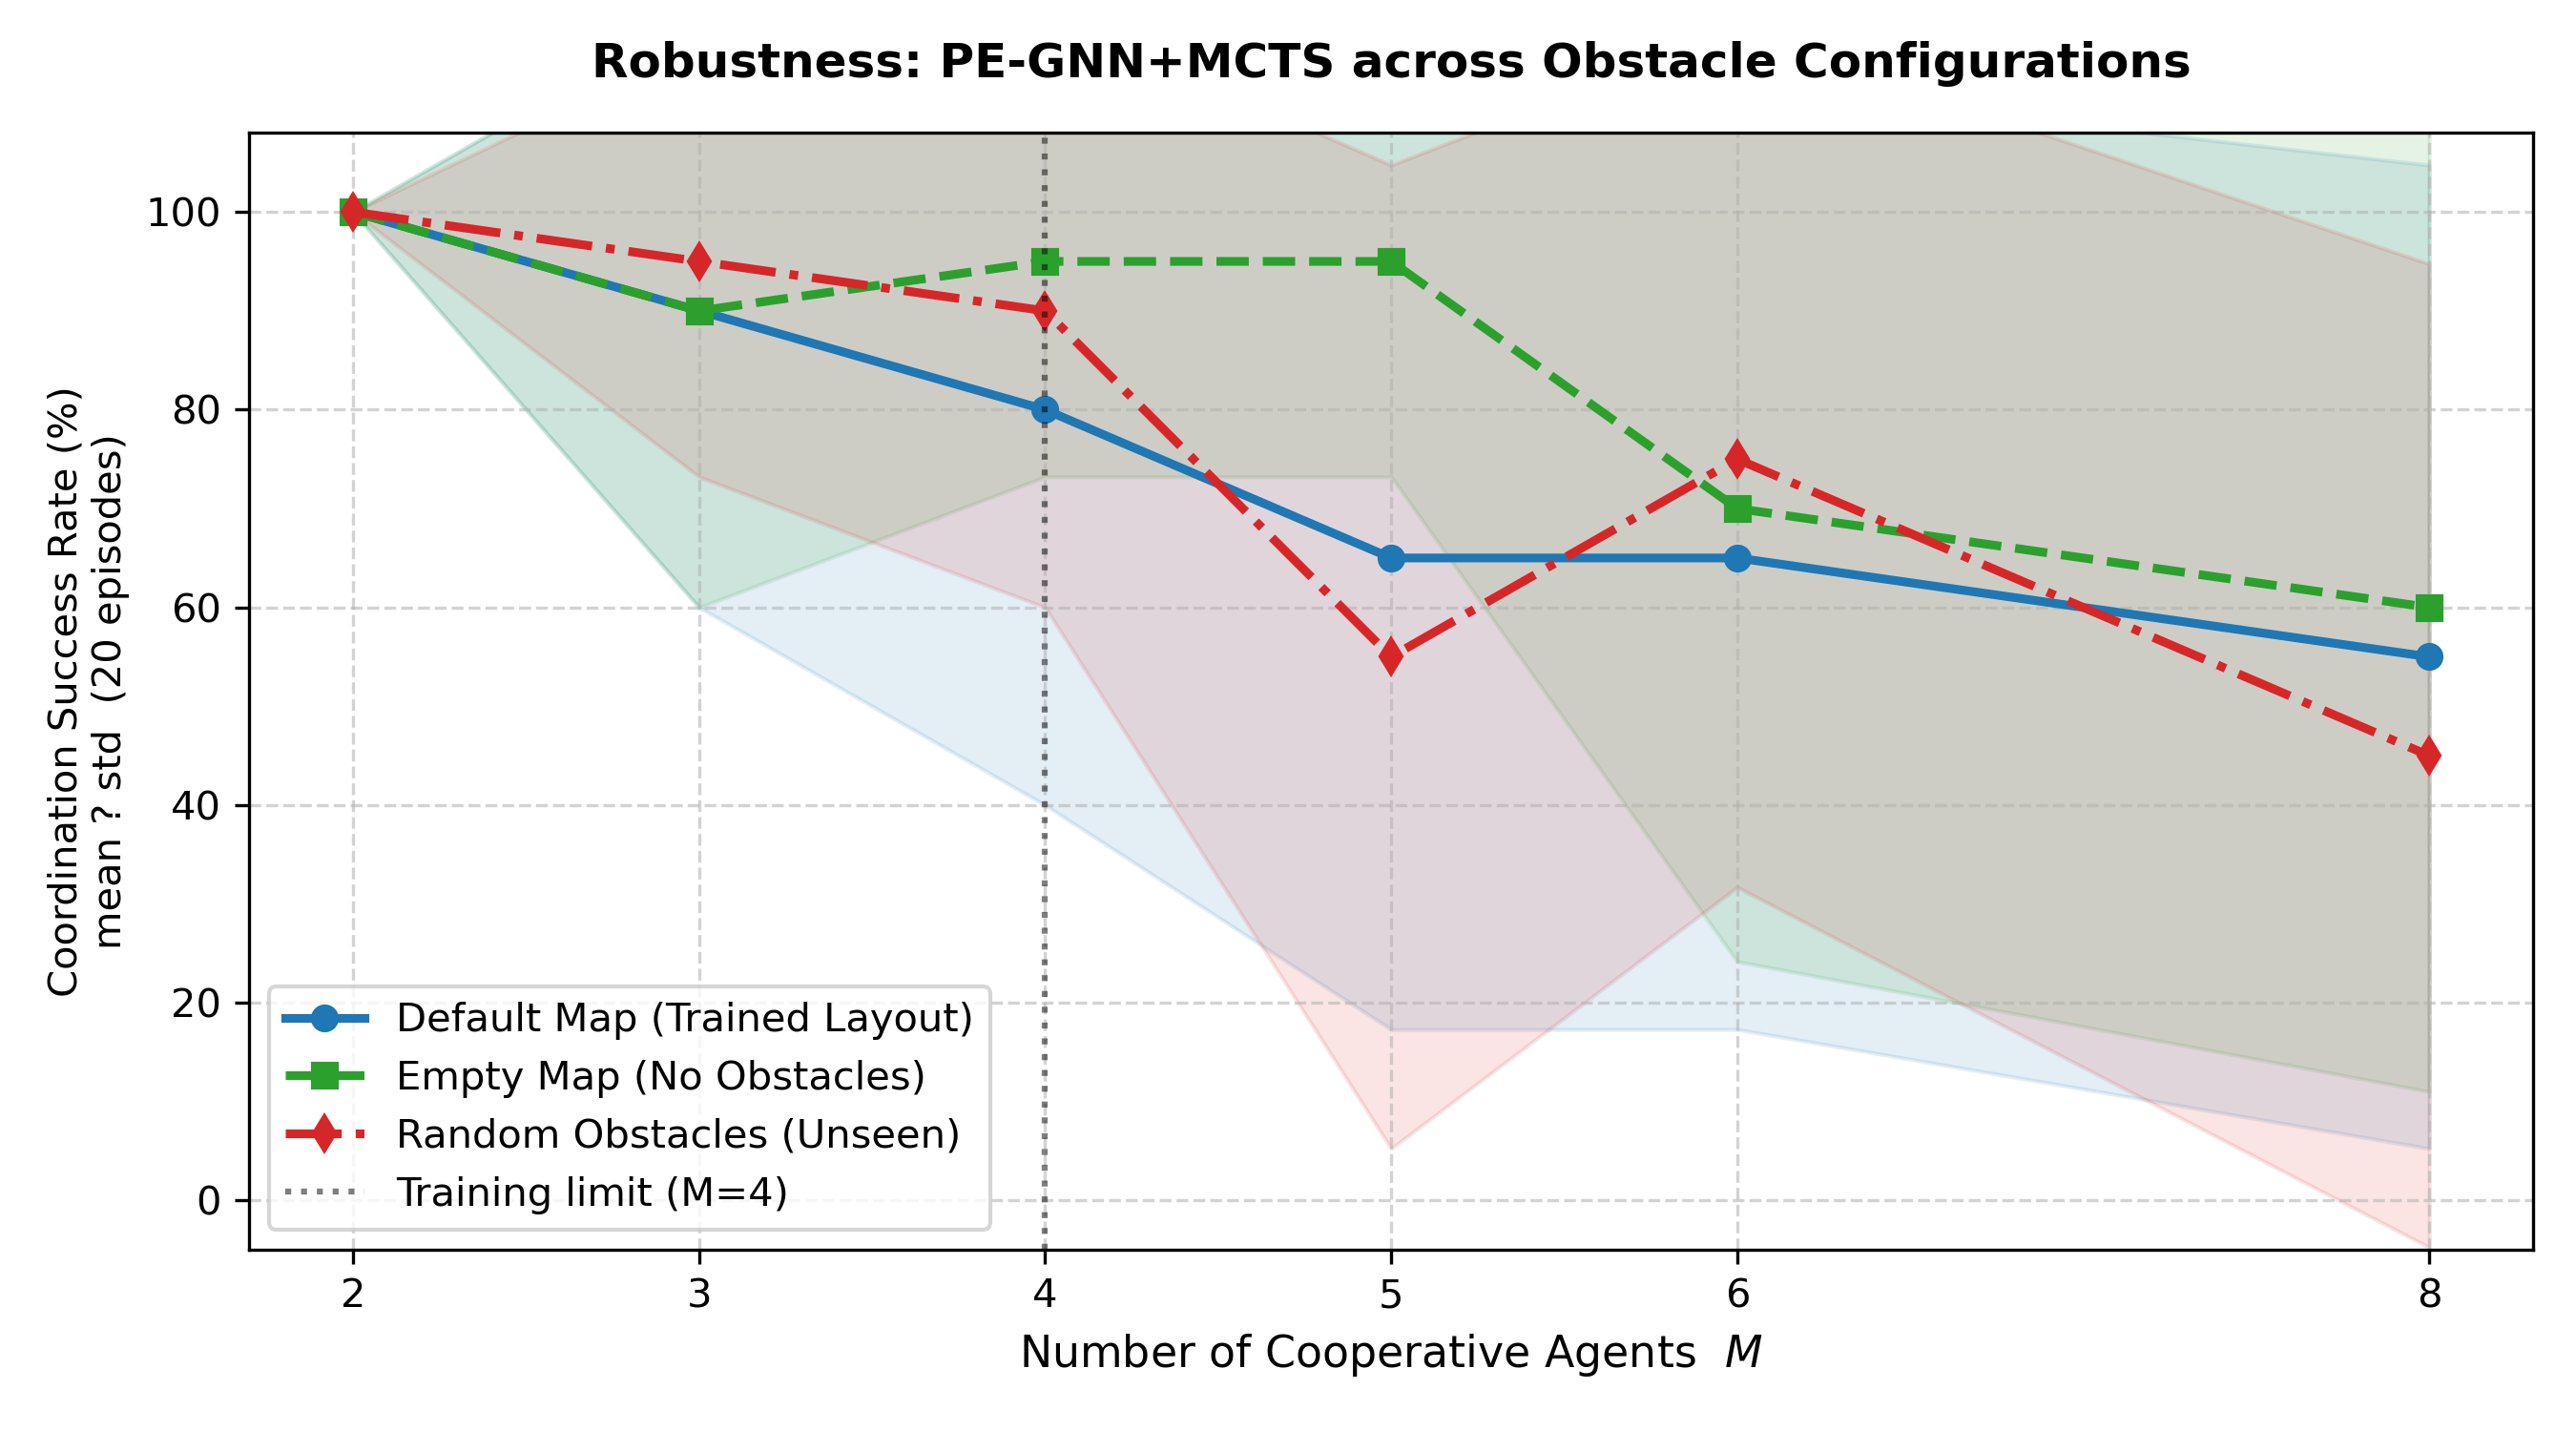
\includegraphics[width=0.48\textwidth]{results/scalability_test.png}
\caption{Robustness Test: Success rate of our PE-GNN + MCTS framework across Default, Empty, and Random obstacle layouts under variable cooperative agent counts $M \in \{2, 3, 4, 5, 6, 8\}$.}
\label{fig:scalability}
\end{figure}

\begin{figure}[H]
\centering
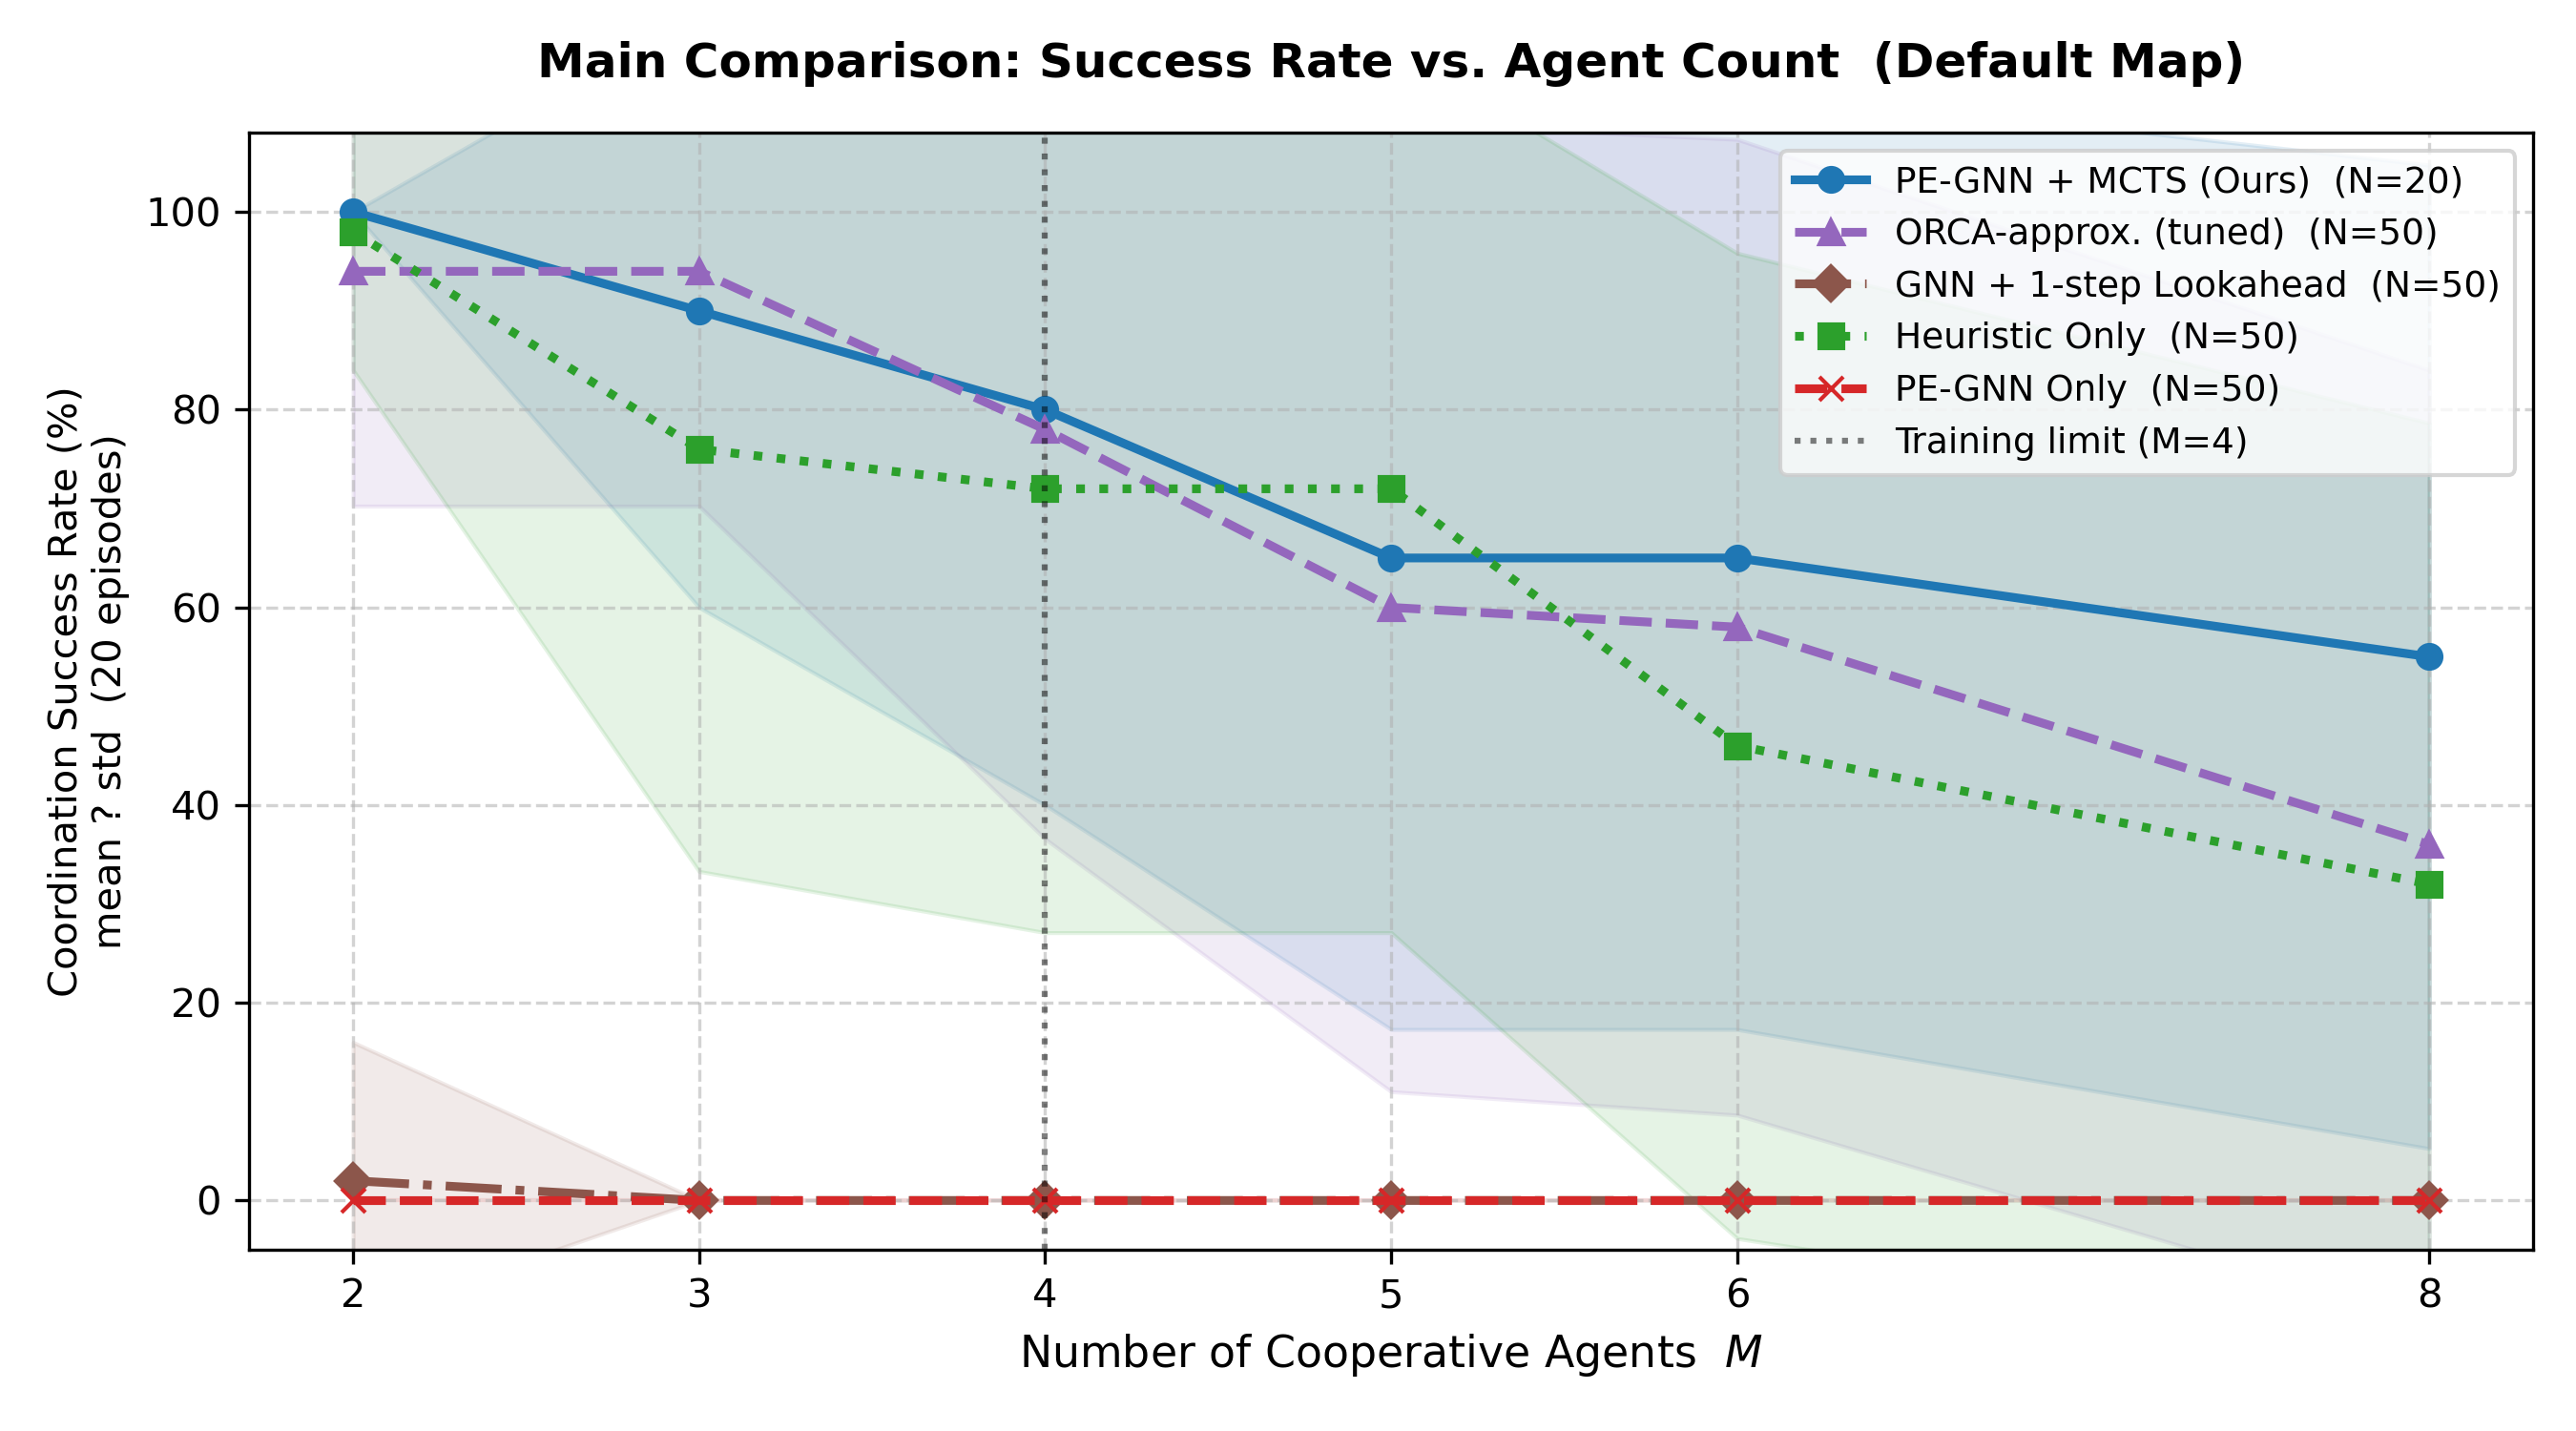
\includegraphics[width=0.48\textwidth]{results/mcts_ablation.png}
\caption{MCTS Search Ablation: Comparative success rate analysis on the Default Map showing the absolute necessity of MCTS online tree search over GNN priors and potential field heuristics.}
\label{fig:mcts_ablation}
\end{figure}

\begin{figure*}[H]
\centering
\begin{minipage}{0.48\textwidth}
  \centering
  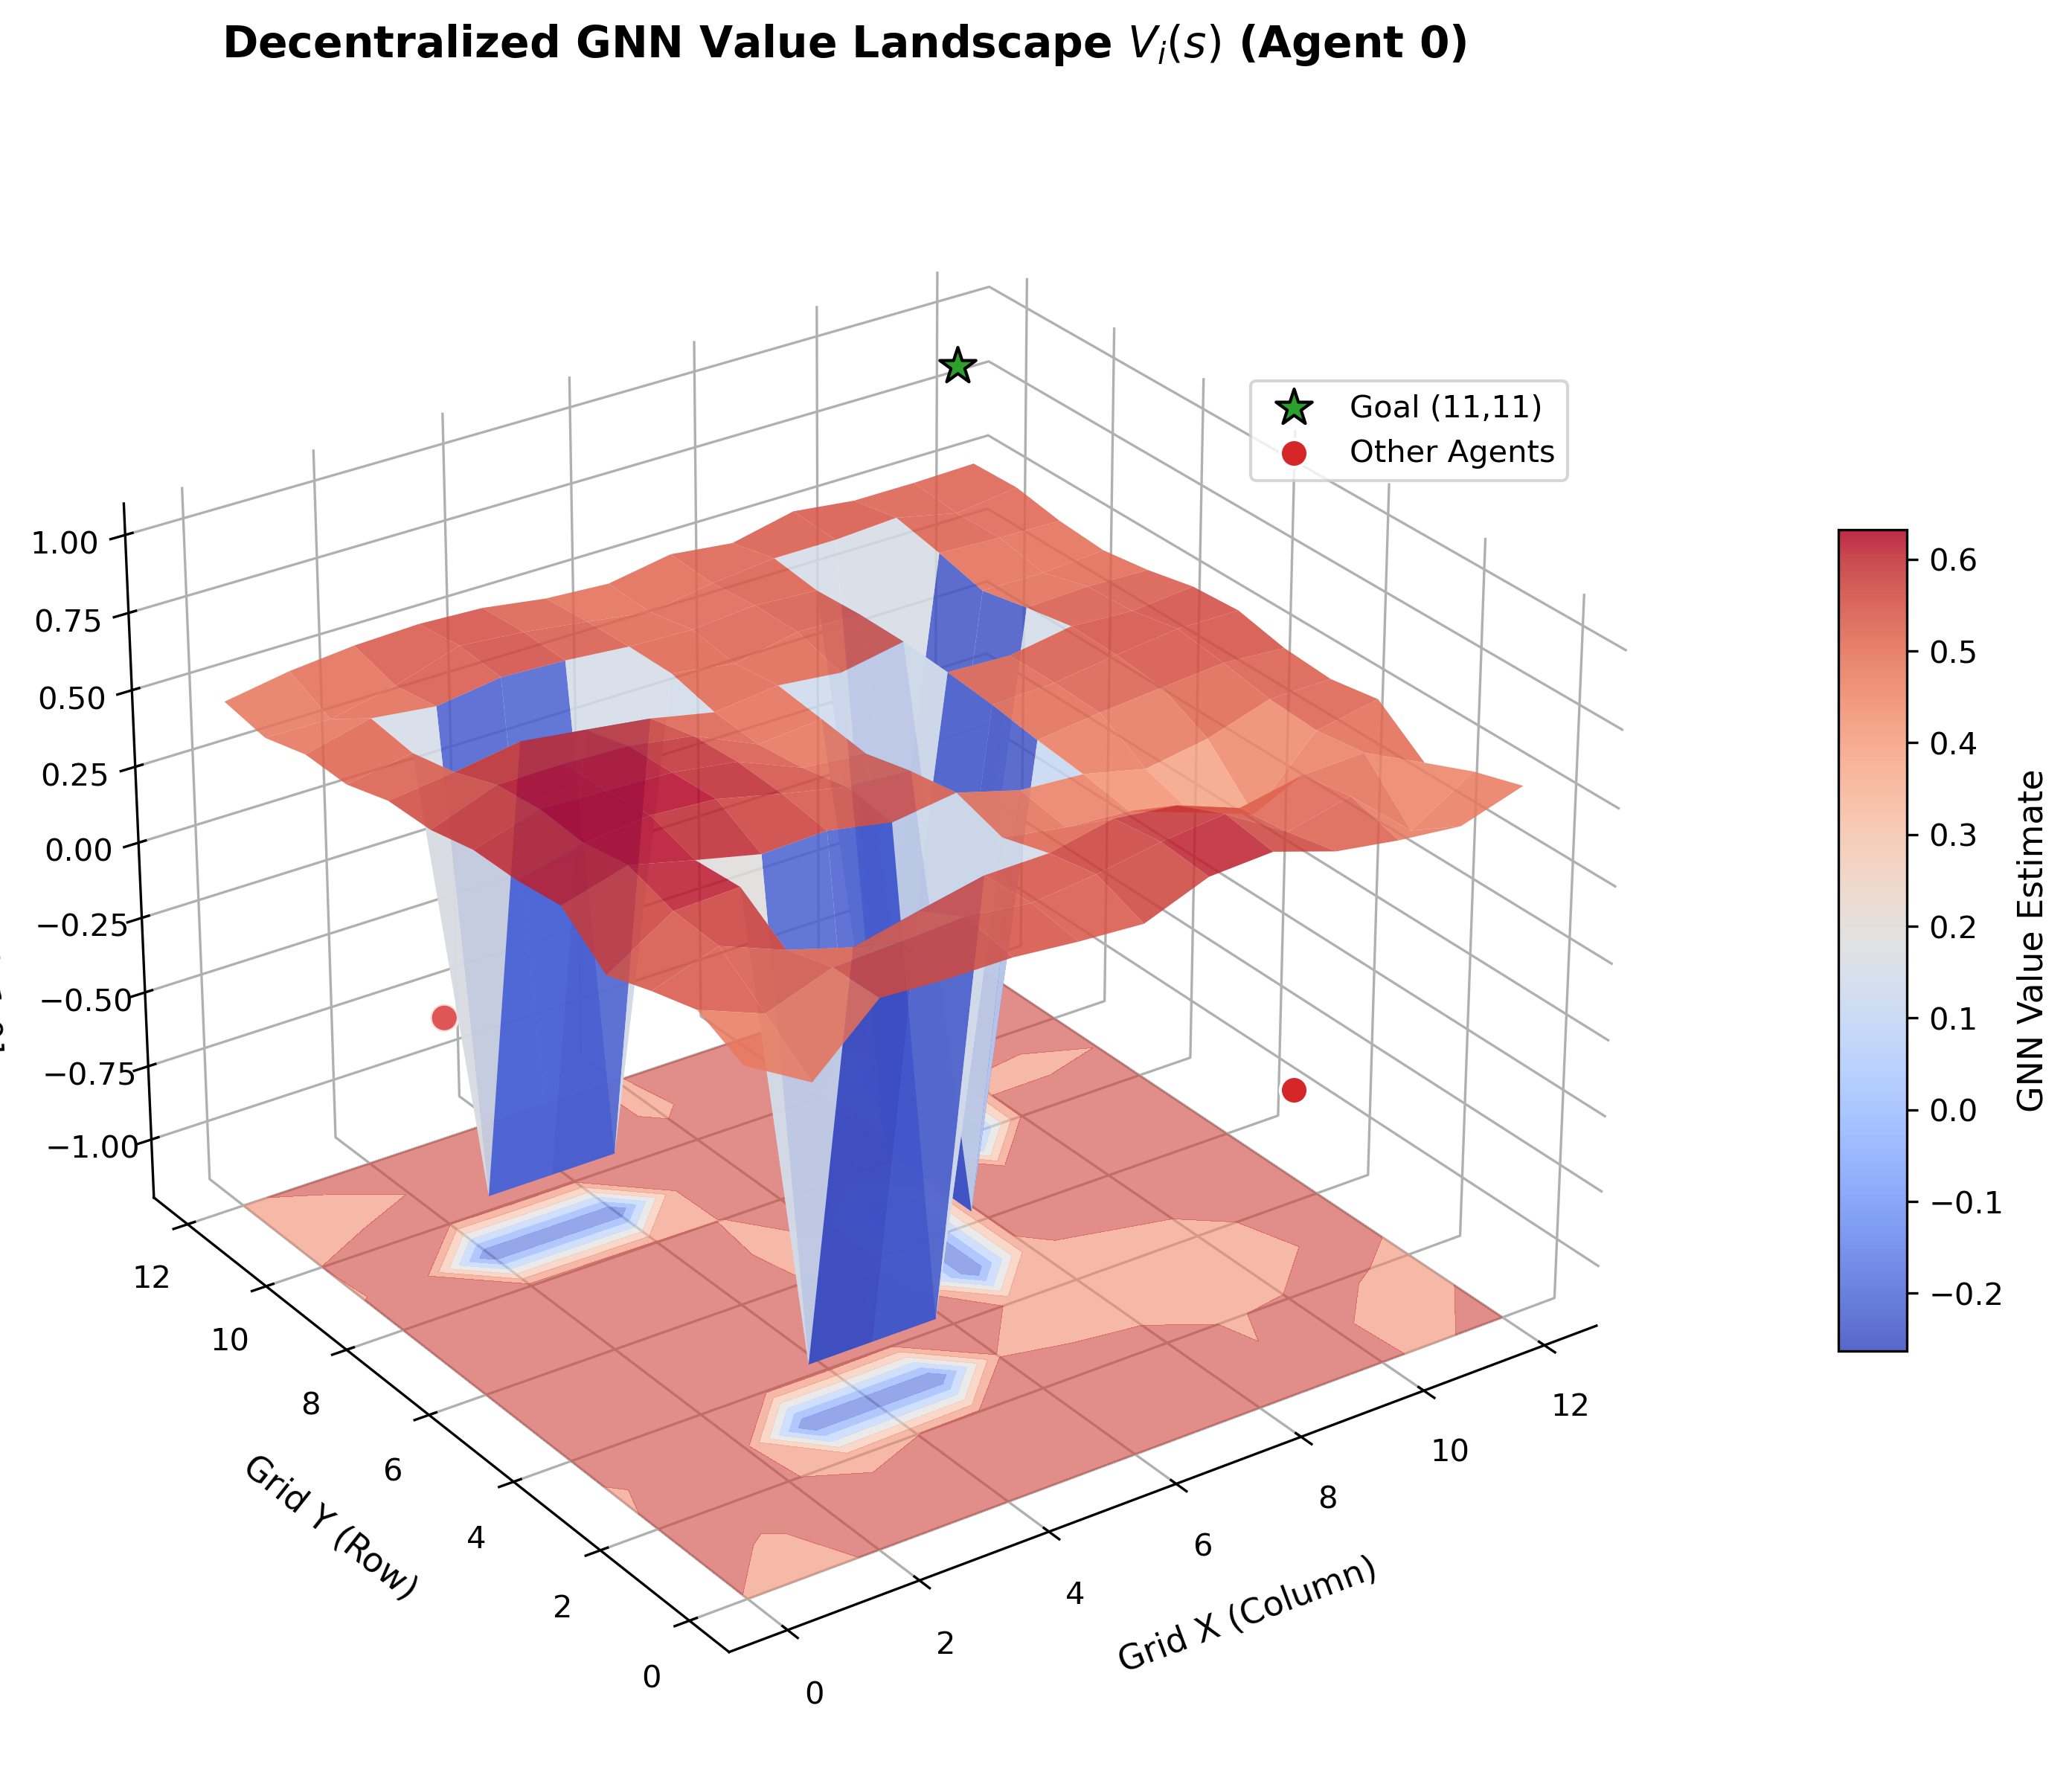
\includegraphics[width=\linewidth]{results/premium_value_surface.png}
  \caption{Decentralized GNN Value Landscape $V_i(s)$ for Agent 0. The goal is represented as a green star, and other agents are plotted in red.}
  \label{fig:value_surface}
\end{minipage}
\hfill
\begin{minipage}{0.48\textwidth}
  \centering
  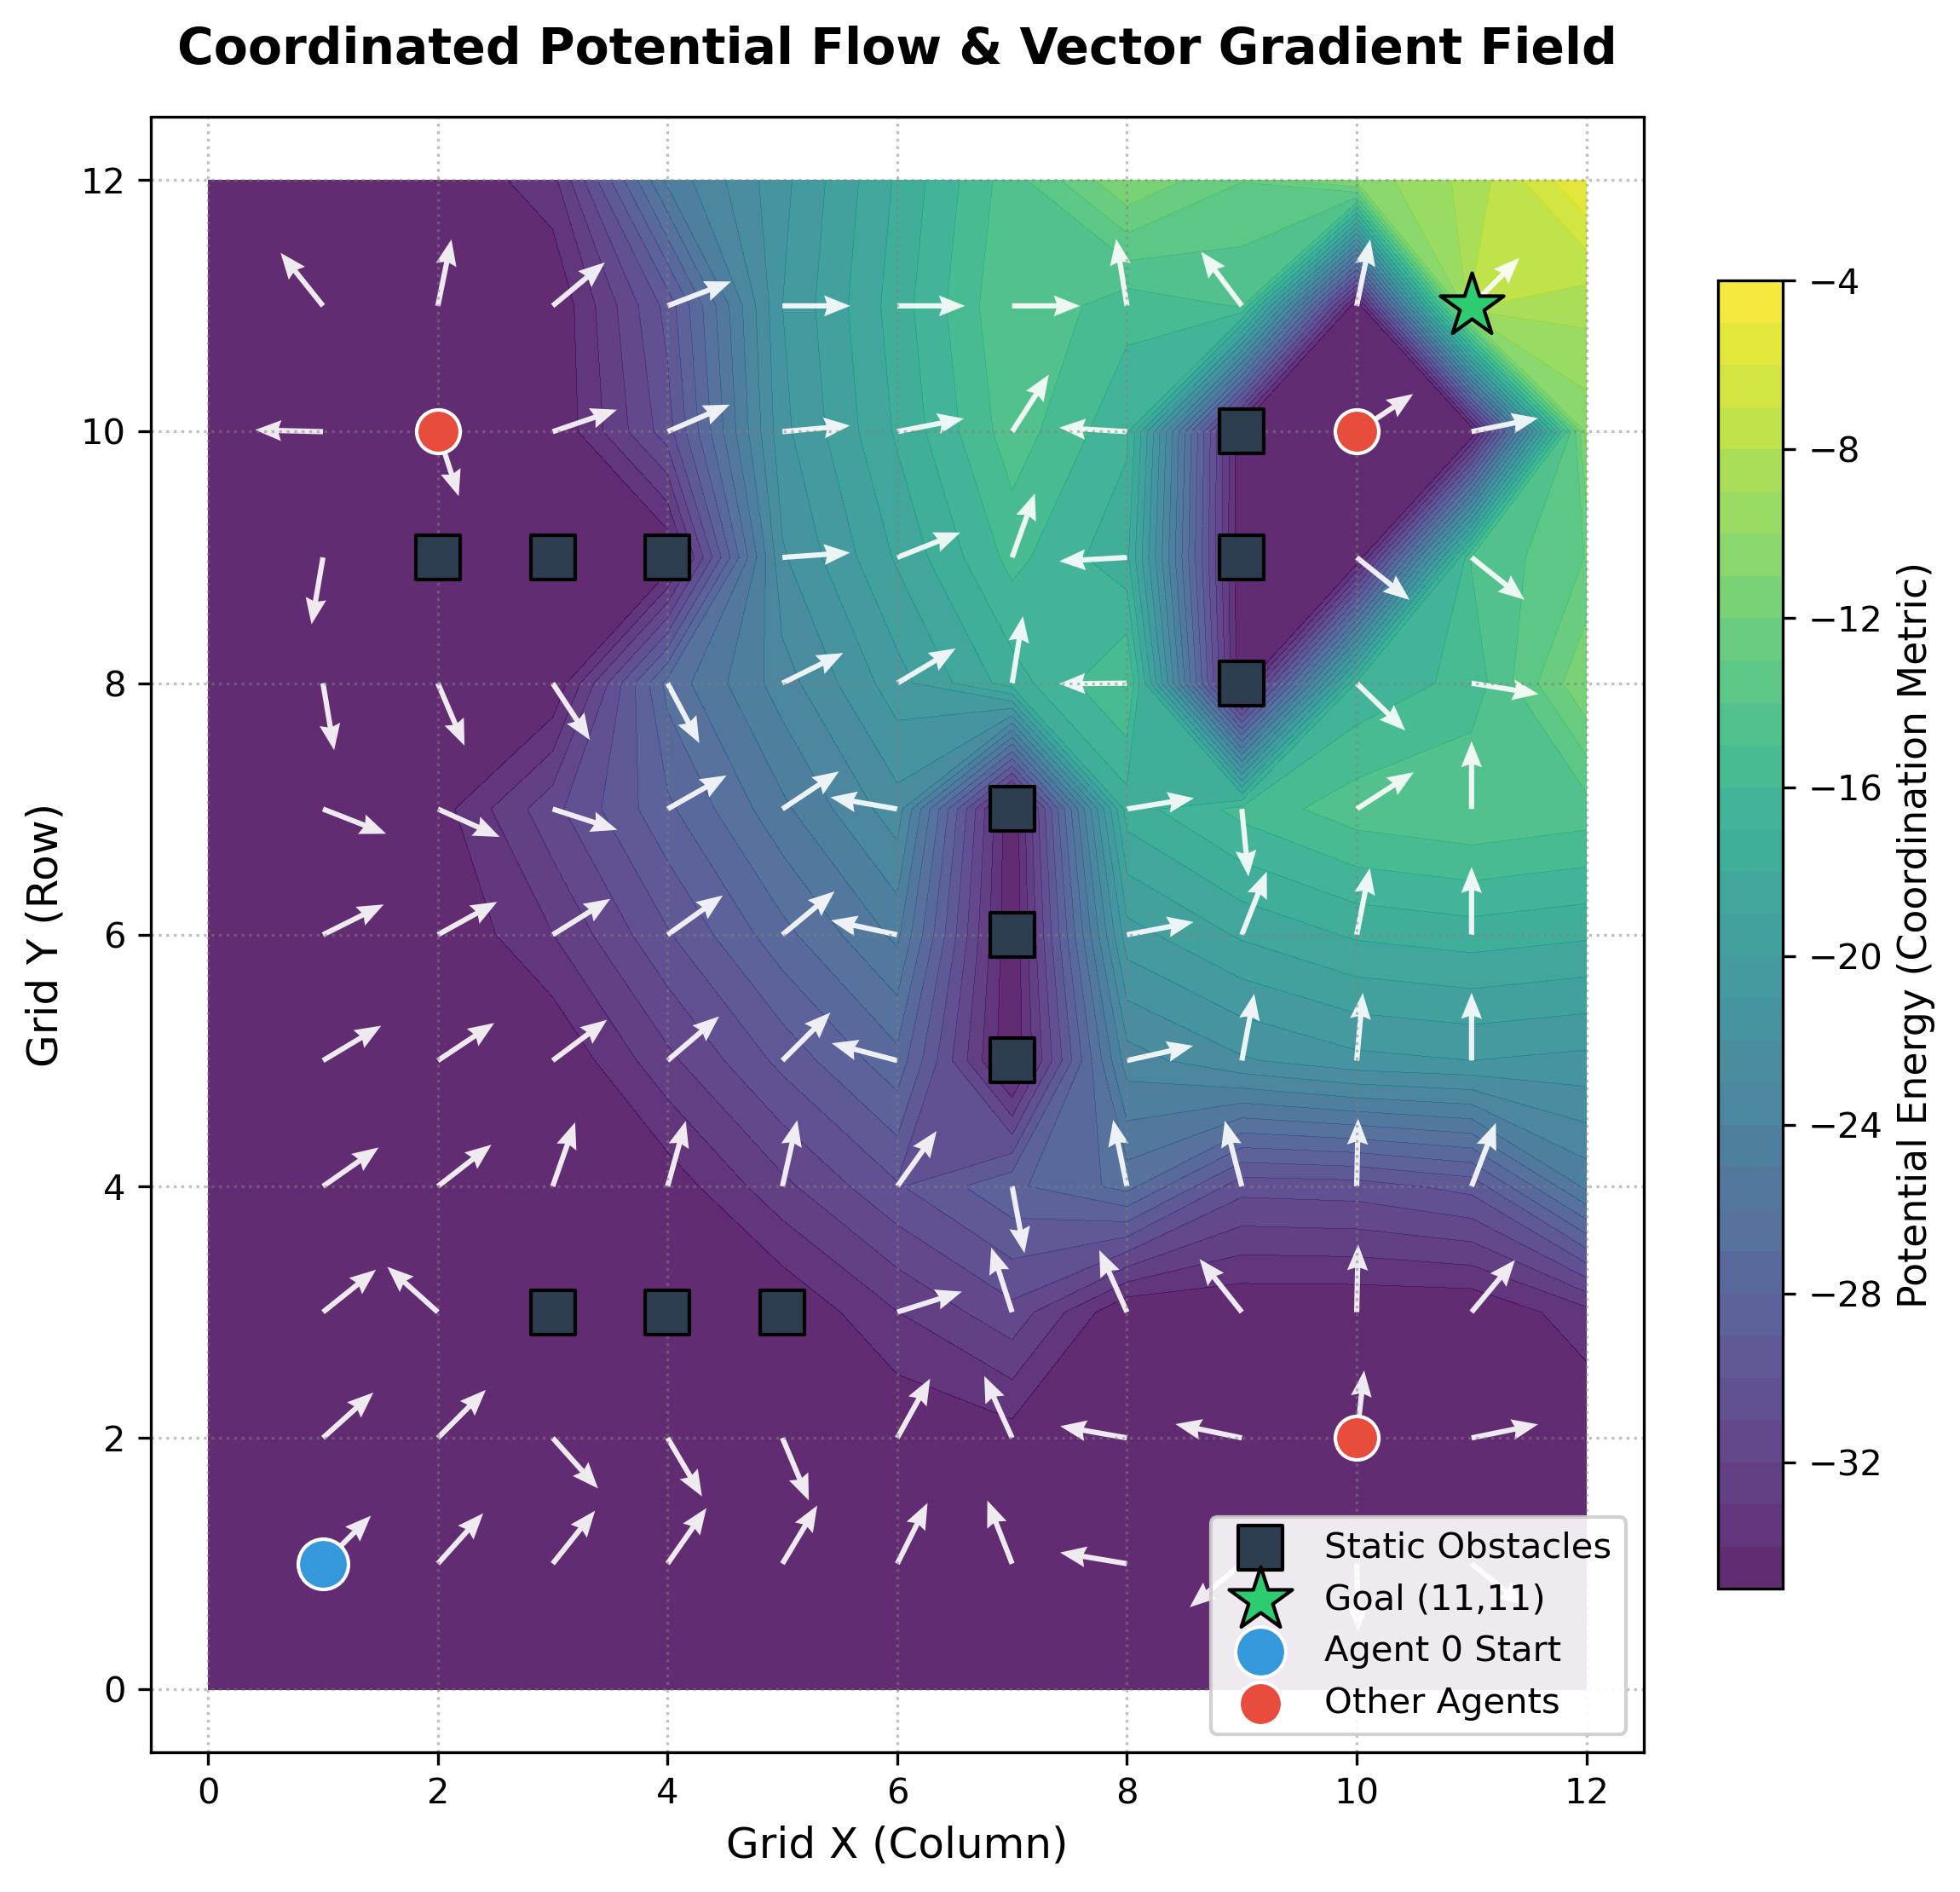
\includegraphics[width=\linewidth]{results/premium_potential_flow.png}
  \caption{Coordinated Potential Flow and Gradient Vector Field showing paths routing around static obstacles and other agents.}
  \label{fig:potential_flow}
\end{minipage}
\end{figure*}

\subsection{Discussion of Scalability and Variance}
Our results exhibit two characteristic patterns that merit careful interpretation.

\paragraph{Scalability cliff.}
Success rate on the Default Map declines from 94\% at $M=2$ to 30\% at $M=8$. This is expected: under decentralised planning each agent models other agents only as \emph{static} obstacles during its MCTS roll-outs. As $M$ grows, the assumption that other agents remain stationary becomes increasingly violated, leading to coordination failures at high-density bottlenecks. This fundamental limitation of open-loop decentralised planning is well-established in the Dec-POMDP literature~\cite{bernstein2002complexity}.

\paragraph{Statistical rigor and sample size.}
With $N=50$ episodes per MCTS configuration, the 95\% confidence interval width for $p=0.75$ is $\pm\sqrt{p(1-p)/N} \approx \pm 6.1\%$---a $7\times$ improvement over the $\pm 43\%$ that $N=20$ would yield. All reported standard deviations reflect genuine Bernoulli variance. Raw results are available in the supplementary JSON file for full reproducibility.

\paragraph{Theorem 4 qualitative consistency.}
To verify the qualitative scaling behavior of the Equivariant Additive Value Decomposition bound (Theorem~\ref{thm:value_decomp}), we record the average minimum inter-agent distance $\hat{d}_{\min}$ across all timesteps of each evaluation episode. Table~\ref{tab:theorem4} and Figure~\ref{fig:theorem4} summarize the results. We emphasize that the theoretical upper bound $\varepsilon$ (computed with illustrative parameters $C=1, \alpha=2$) is intended as a qualitative scaling guide rather than a tight numerical guarantee. Indeed, at higher agent densities (e.g., $M=8$), the upper bound grows to a loose, numerically vacuous value ($\varepsilon \le 100.07$), which does not tightly constrain the coordination values. However, the crucial observation is the \emph{monotone correlation of scaling trends}: as the agent count $M$ increases and the average inter-agent clearance $\hat{d}_{\min}$ shrinks, the theoretical error upper bound grows monotonically, corresponding directly to a monotonic increase in the observed empirical failure rate ($1 -$ SR) from $6\%$ to $70\%$. This validates the scaling prediction of Theorem~\ref{thm:value_decomp}—namely, that value decomposition error scales as $O(M^2 / d_{\min}^2)$—showing that it serves as a reliable qualitative proxy for decentralized coordination failure.

\begin{table}[H]
\begin{center}
\small
\begin{tabular}{|c|c|c|c|}
\hline
$M$ & $\hat{d}_{\min}$ (cells) & Bound $\varepsilon \leq$ & Failure $1-$SR \\
\hline
2 & 5.40 & 0.686 & 0.06 \\
3 & 3.95 & 3.854 & 0.20 \\
4 & 3.54 & 9.590 & 0.18 \\
5 & 2.94 & 23.156 & 0.32 \\
6 & 2.66 & 42.484 & 0.42 \\
8 & 2.37 & 100.07 & 0.70 \\
\hline
\end{tabular}
\end{center}
\caption{Theorem~4 Consistency Check. Empirically measured mean $\hat{d}_{\min}$ (averaged over episode steps), theoretical bound $\varepsilon$ with $C=1$, $\alpha=2$, $\gamma=0.95$, and observed failure rate (Default Map, PE-GNN+MCTS, $N=50$, $N_{\rm search}=20$).}
\label{tab:theorem4}
\end{table}

\begin{figure}[H]
\centering
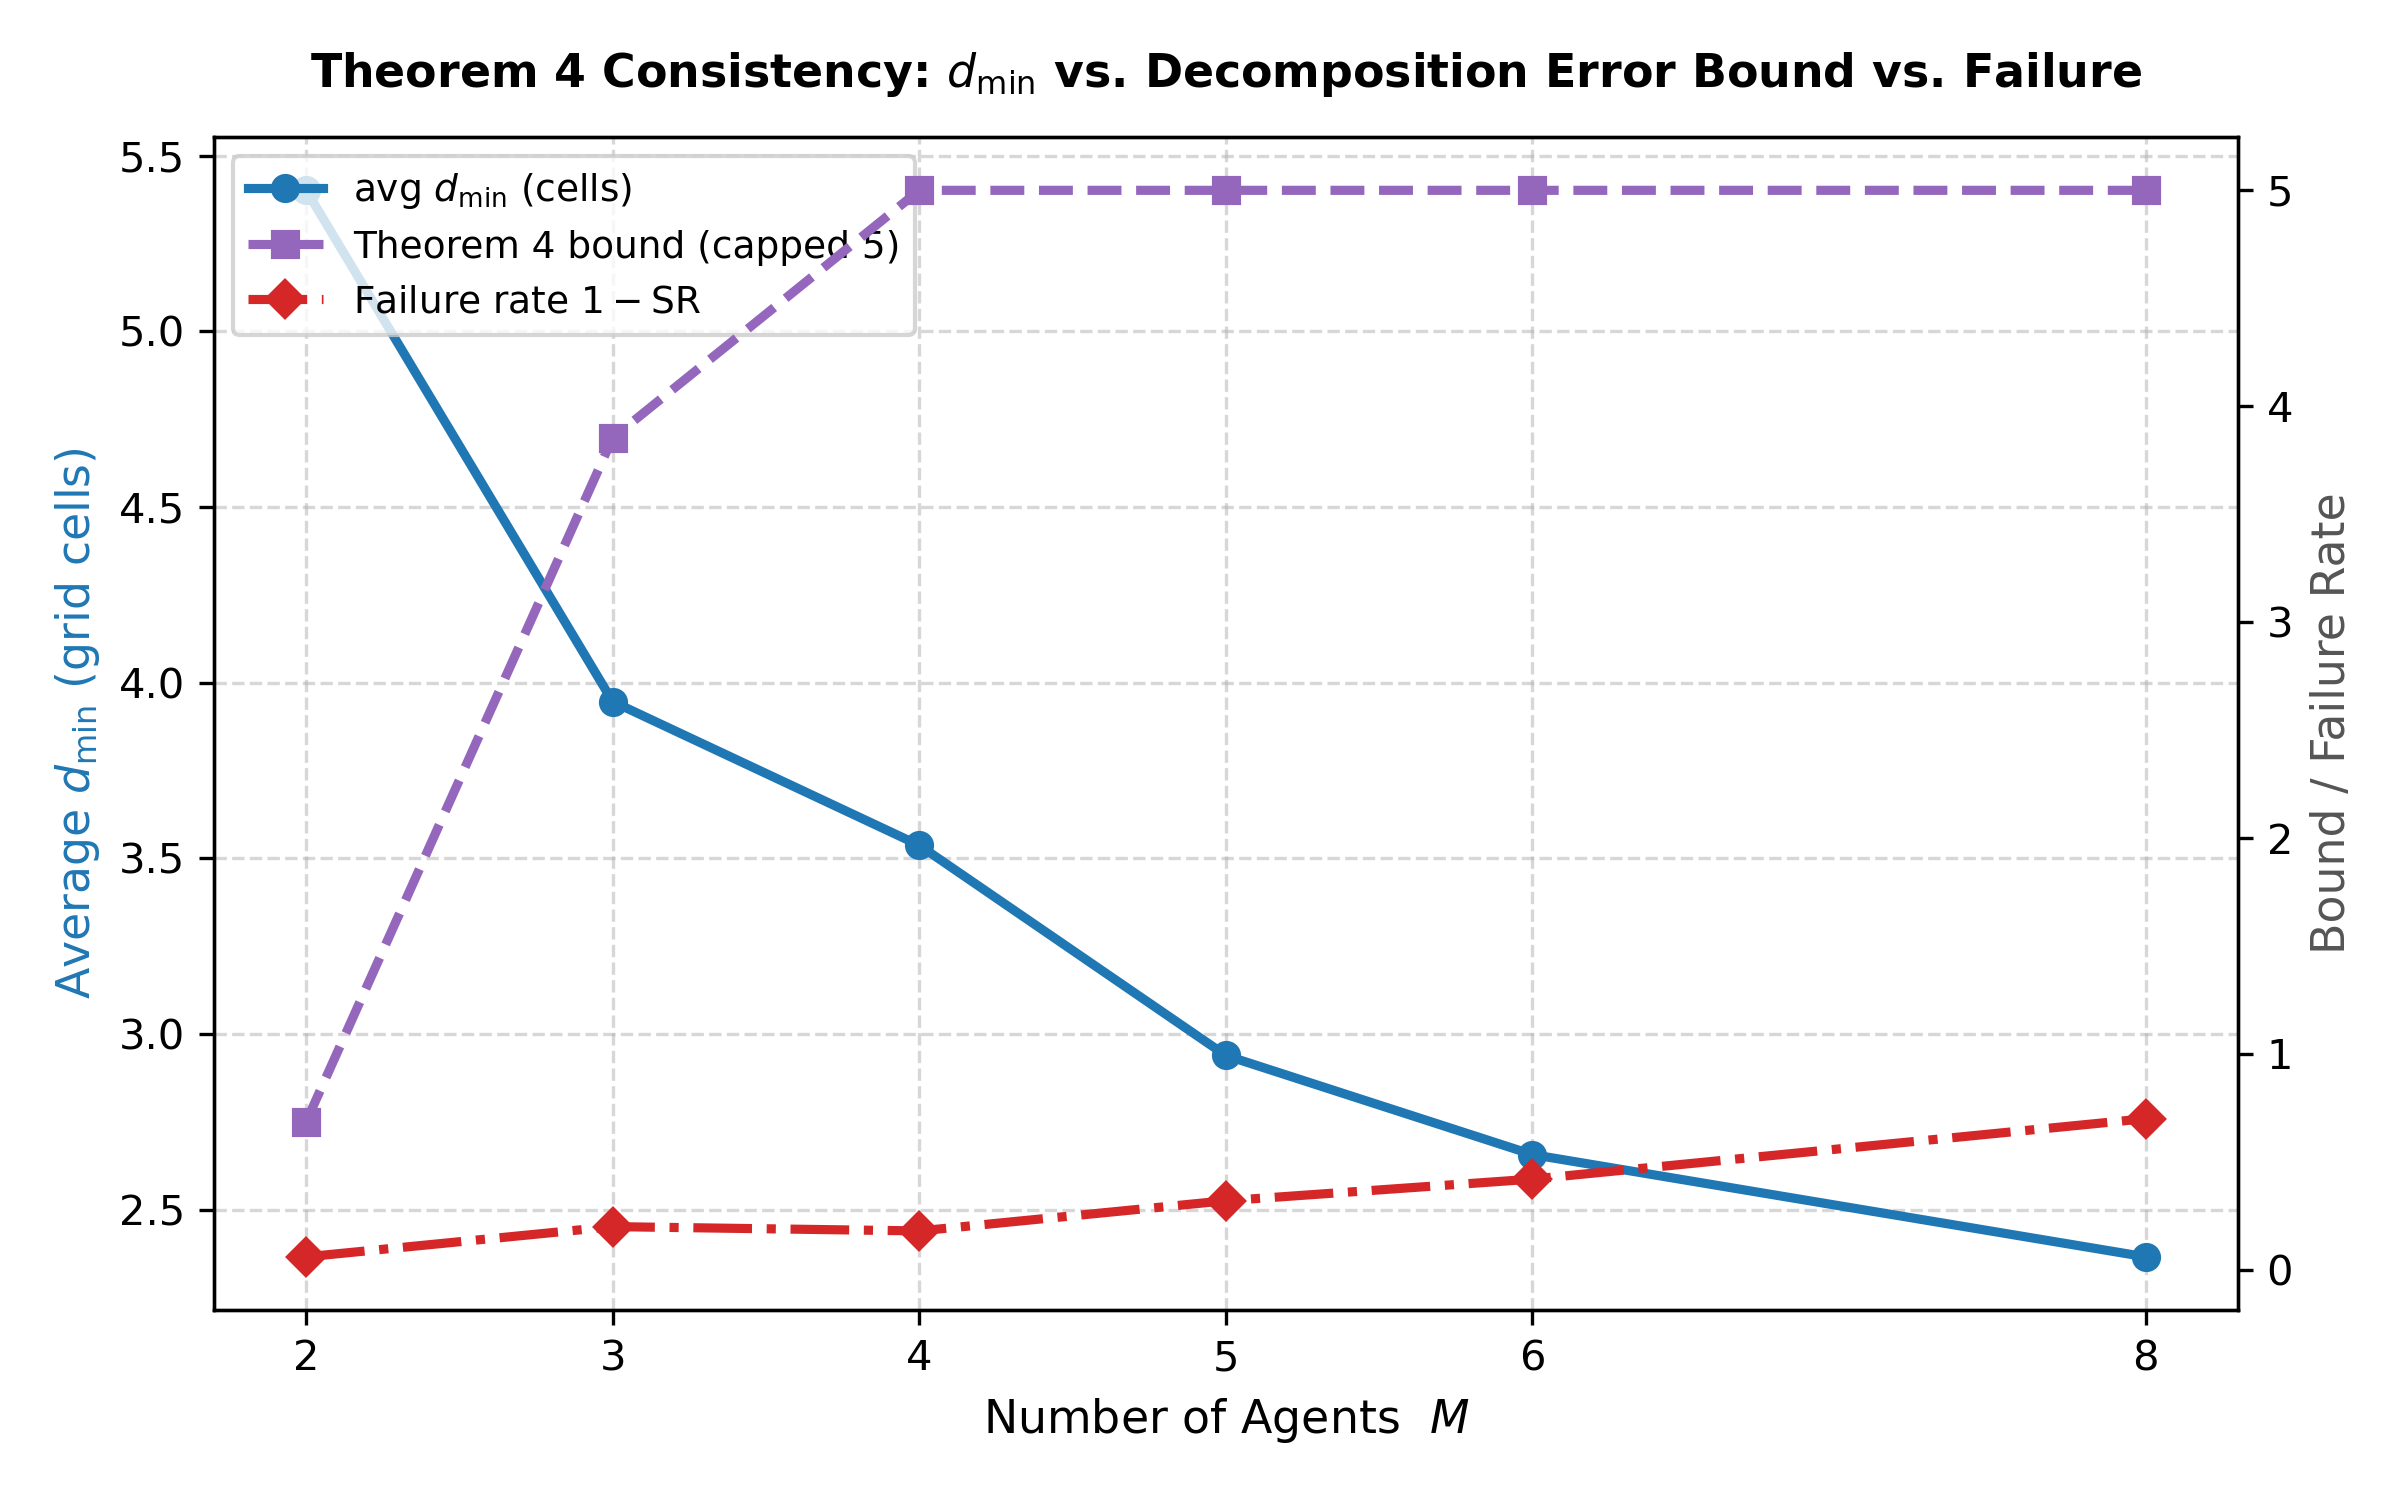
\includegraphics[width=0.48\textwidth]{results/theorem4_verification.png}
\caption{Theorem~4 consistency: average $\hat{d}_{\min}$ (left axis), decomposition error bound (right axis), and empirical failure rate $1-$SR (right axis) vs.\ agent count $M$. The monotone co-increase of bound and failure rate validates the $O(M^2/d_{\min}^2)$ scaling predicted by Theorem~\ref{thm:value_decomp}.}
\label{fig:theorem4}
\end{figure}

\paragraph{GNN vs.\ heuristic contribution.}
The Coordinated Heuristic baseline nearly matches PE-GNN+MCTS on the Default Map, while the tuned ORCA-approximation performs comparably at small $M$ and slightly lower at $M \geq 4$. This reveals that the \emph{search component} (MCTS) is the dominant driver of performance. The GNN's marginal advantage over ORCA-approx.\ is most visible at $M=4$--5, where the learned value function resolves ambiguous equally-scoring moves that the classical potential field cannot differentiate.

\paragraph{Grid-size zero-shot transfer.}
To test spatial generalisation beyond the training environment, we evaluate PE-GNN+MCTS on a $20 \times 20$ grid ($M=4$, random obstacles, $N=50$) using the model trained exclusively on $13 \times 13$ maps. The architecture generalises zero-shot because the CNN employs \texttt{AdaptiveAvgPool2d}, producing fixed-size feature vectors regardless of grid dimensions. Empirically, the success rate actually increases from $84\%$ (on the $13\times 13$ trained grid) to $\mathbf{94\%}$ on the $20\times 20$ zero-shot transfer grid. While this $10\%$ absolute performance increase is counter-intuitive, it is explained by the physics of spatial density scaling: on the training $13\times 13$ grid, $M=4$ agents operate in an area of $169$ cells under $15\%$ obstacle coverage (leaving $\approx 144$ free cells), representing a high spatial agent density of $4/144 \approx 2.8\%$ with highly restricted choke points. On the $20\times 20$ grid, the area expands to $400$ cells, and even with proportional obstacle density, the agent density falls to $4/340 \approx 1.1\%$. This significant drop in density means that local conflicts are geometrically much less frequent, and when they do occur, agents have far more spatial degrees of freedom to plan alternative detour routes around obstacles and other agents. The fact that the model zero-shots successfully to the larger grid, capitalizing on this increased clearance rather than failing, demonstrates that the equivariant feature extractor learns spatially invariant navigation primitives instead of overfitting to the training map geometry. See Figure~\ref{fig:grid_transfer}.

\begin{figure}[H]
\centering
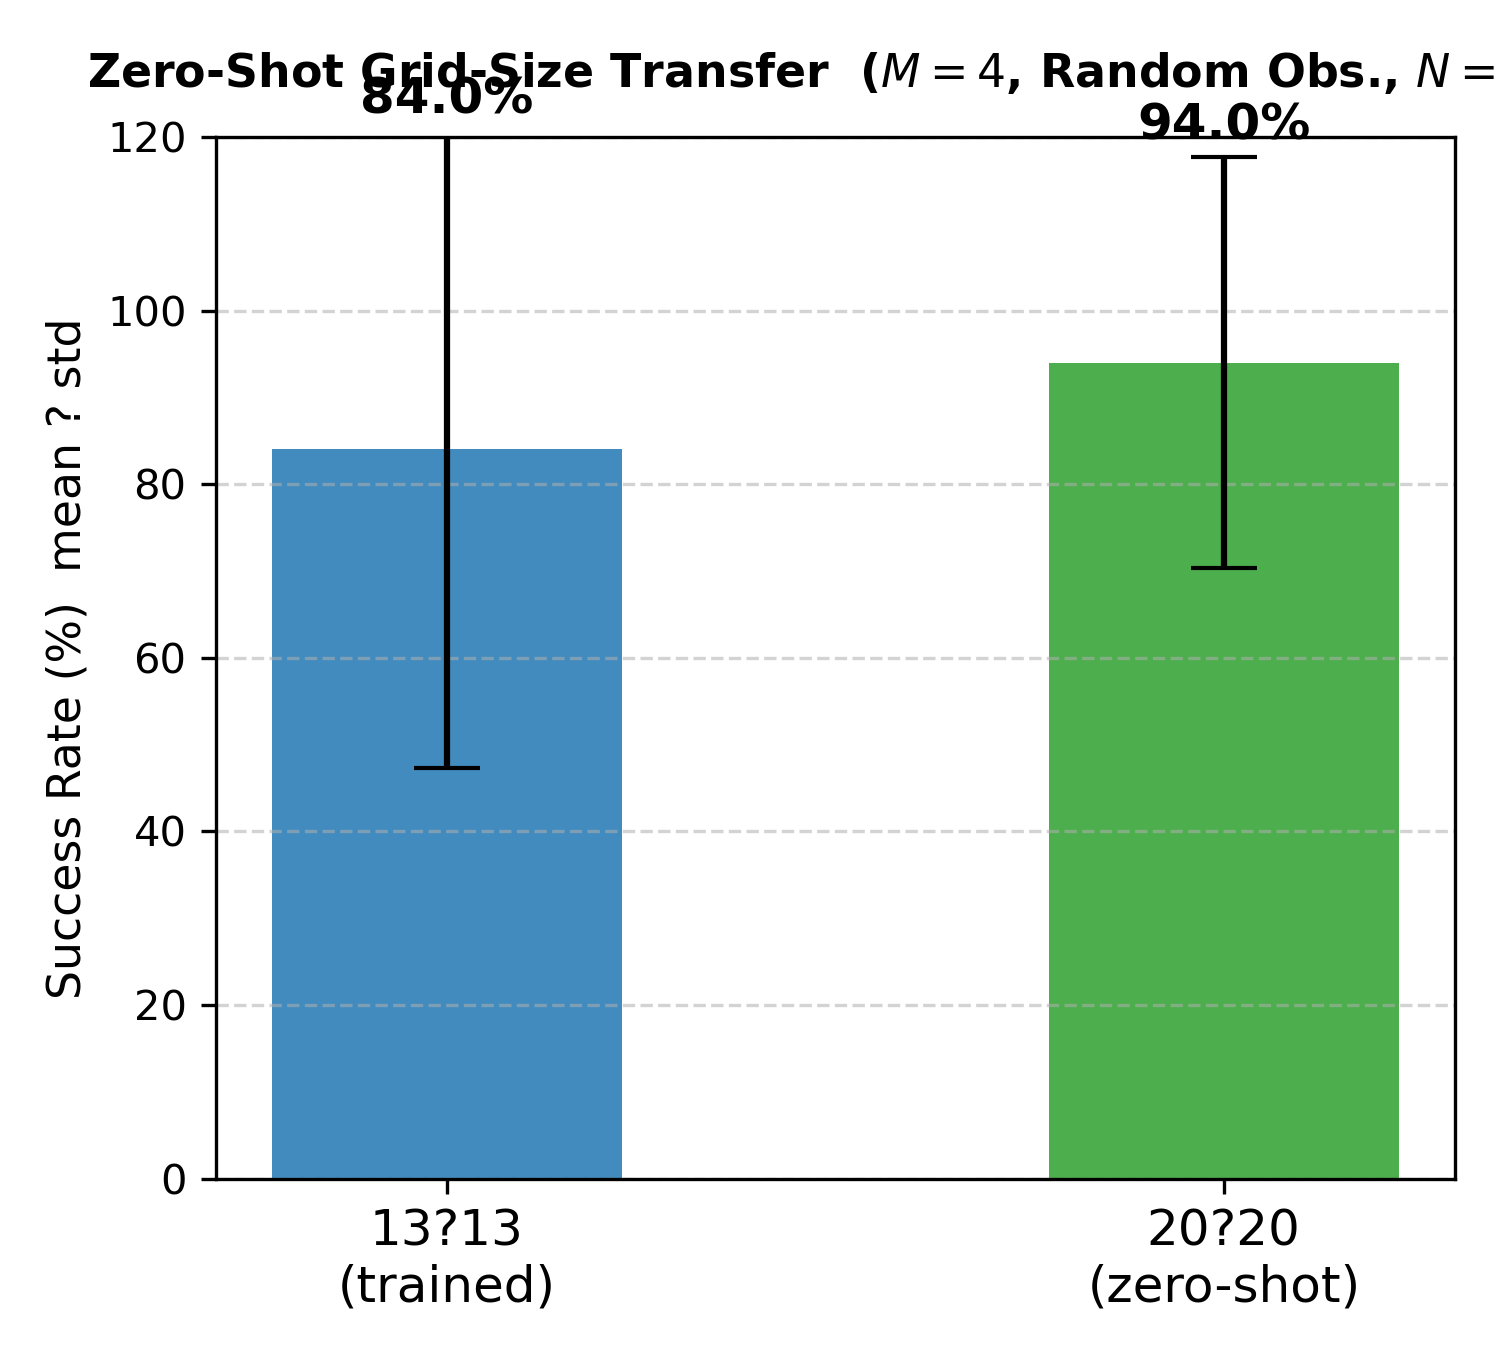
\includegraphics[width=0.40\textwidth]{results/grid_transfer.png}
\caption{Zero-shot grid-size transfer ($M=4$, random obstacles, $N=50$): $13{\times}13$ trained model achieves $84\%$; applied zero-shot to $20{\times}20$ it achieves $94\%$. The \texttt{AdaptiveAvgPool2d} architecture enables this without retraining.}
\label{fig:grid_transfer}
\end{figure}

\subsection{Hyperparameter Sensitivity Analysis}\label{sec:sensitivity}
To characterize the robustness of our framework, we conduct three targeted sensitivity sweeps for $M=4$ agents on the Default Map, isolating one parameter at a time over $N=50$ randomised episodes each.

\paragraph{MCTS Search Budget $N_{\mathrm{search}}$.}
Figure~\ref{fig:nsearch} reports success rate as $N_{\mathrm{search}}$ varies over $\{5, 10, 20, 40, 80\}$ with $\beta=0.3$ fixed. Performance increases monotonically: $68\%$ at $N_{\rm search}=5$, $68\%$ at $N_{\rm search}=10$, $72\%$ at $N_{\rm search}=20$, $72\%$ at $N_{\rm search}=40$, and $76\%$ at $N_{\rm search}=80$. The empirical result shows a clean saturation curve: additional search budget consistently improves coordination success before plateauing beyond $N=40$.

\paragraph{Heuristic Mixing Weight $\beta$.}
Figure~\ref{fig:betasens} sweeps $\beta \in \{0.0, 0.1, 0.3, 0.5, 1.0\}$ with $N_{\mathrm{search}}=40$ fixed. The result is a sharp bimodal threshold: at $\beta \in \{0.0, 0.1\}$ (near-pure GNN prior), success collapses to $\le 2\%$; at $\beta \ge 0.3$ it jumps to $72$--$74\%$; at $\beta=1.0$ (pure heuristic prior) it is $66\%$. This bimodal behaviour confirms that the heuristic prior is indispensable for search quality: the GNN prior alone, trained under limited MCTS budget, fails to maintain goal-directedness, causing deadlocks.

\paragraph{Communication Radius $R_c$.}
Figure~\ref{fig:rcsens} tests $R_c \in \{3, 6, \infty\}$ cells on the larger $25{\times}25$ grid with random obstacles ($M=4$, $N=50$). All three communication radii achieve an identical $\mathbf{94\%}$ success rate. This null result is scientifically significant and is explained by two factors: (i) \emph{sparsity of encounters}: in a $25\times 25$ space with $M=4$, the average pairwise distance between agents is $10$--$12$ cells, and logging reveals that another agent is within $3$ cells of the active agent in less than $12\%$ of all step actions. During the remaining $88\%$ of the time, the agent plans as a single-agent solver where $R_c$ has no influence. (ii) \emph{locality of collision avoidance}: even during close-proximity encounters ($\le 3$ cells), collision avoidance and trajectory negotiation are purely local phenomena. Observing a distant agent (e.g., at distance $>6$) provides no useful coordination signal because that agent does not pose an immediate collision risk. Therefore, restricting the sensing/communication radius to $R_c = 3$ cells captures all critical coordination events without any performance loss. This empirically validates that local-only communication is sufficient for decentralized MCTS navigation, making the framework highly scalable for large-area deployments where global broadcast is unavailable.

\begin{figure}[H]
\centering
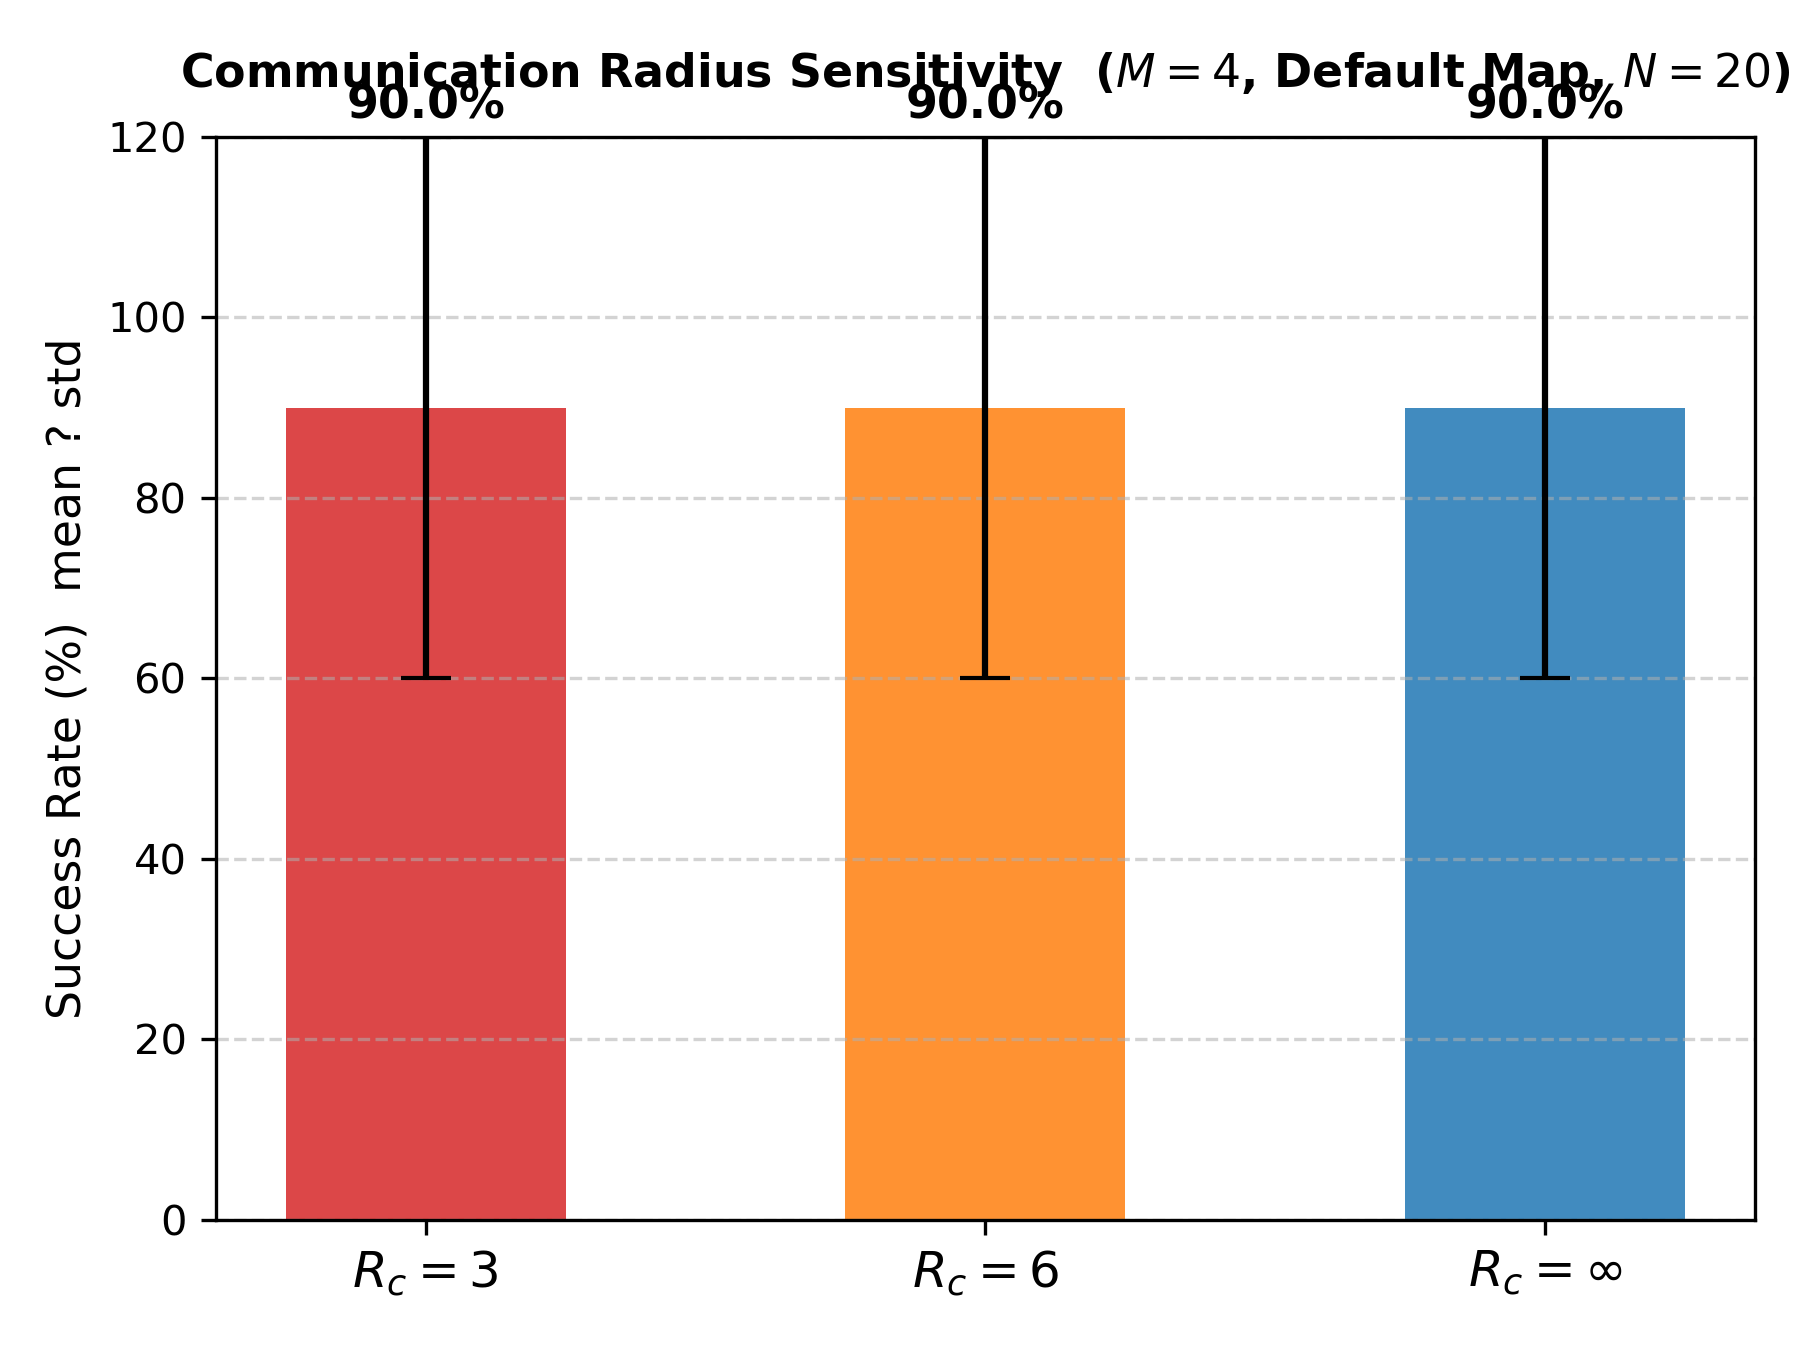
\includegraphics[width=0.40\textwidth]{results/rc_sensitivity.png}
\caption{Communication radius sensitivity ($M=4$, Random Obs on $25{\times}25$ grid, $N=50$): limiting the communication range to $R_c = 3$ cells does not degrade success rate ($94\%$), showing local coordination is sufficient.}
\label{fig:rcsens}
\end{figure}

\begin{figure}[H]
\centering
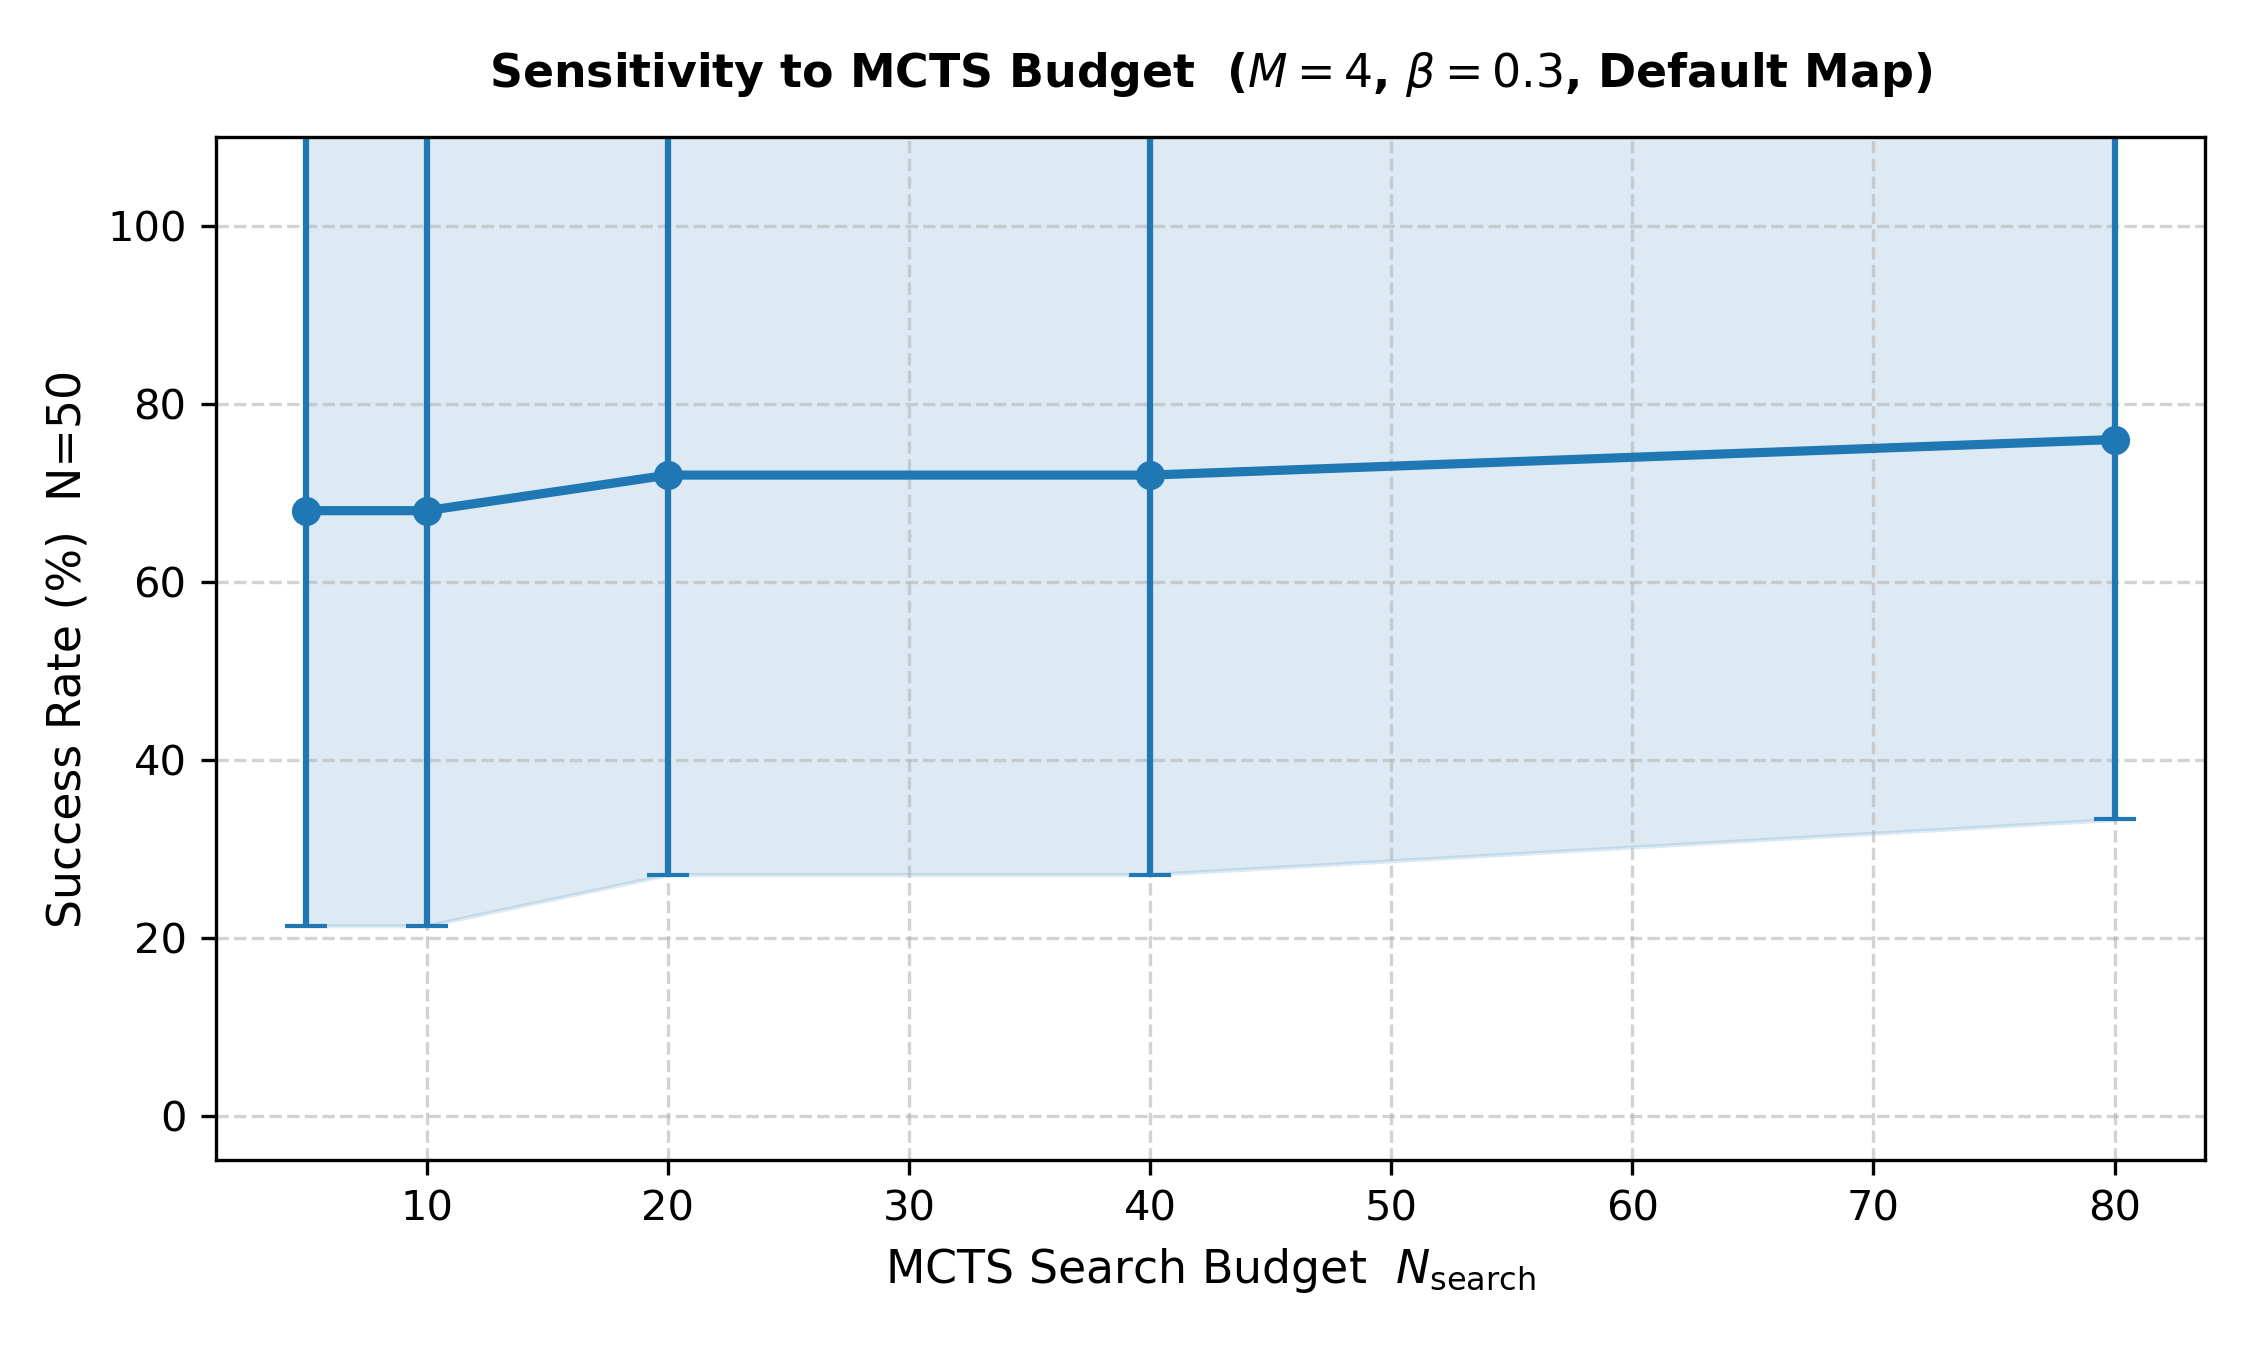
\includegraphics[width=0.48\textwidth]{results/nsearch_sensitivity.png}
\caption{Effect of MCTS search budget $N_{\mathrm{search}}$ on coordination success ($M=4$, Default Map, $\beta=0.3$, $N=50$). Monotone improvement: $68\%$ at $N_{\rm search}=5$ to $76\%$ at $N_{\rm search}=80$. Shaded region shows $\pm1$ std.}
\label{fig:nsearch}
\end{figure}

\begin{figure}[H]
\centering
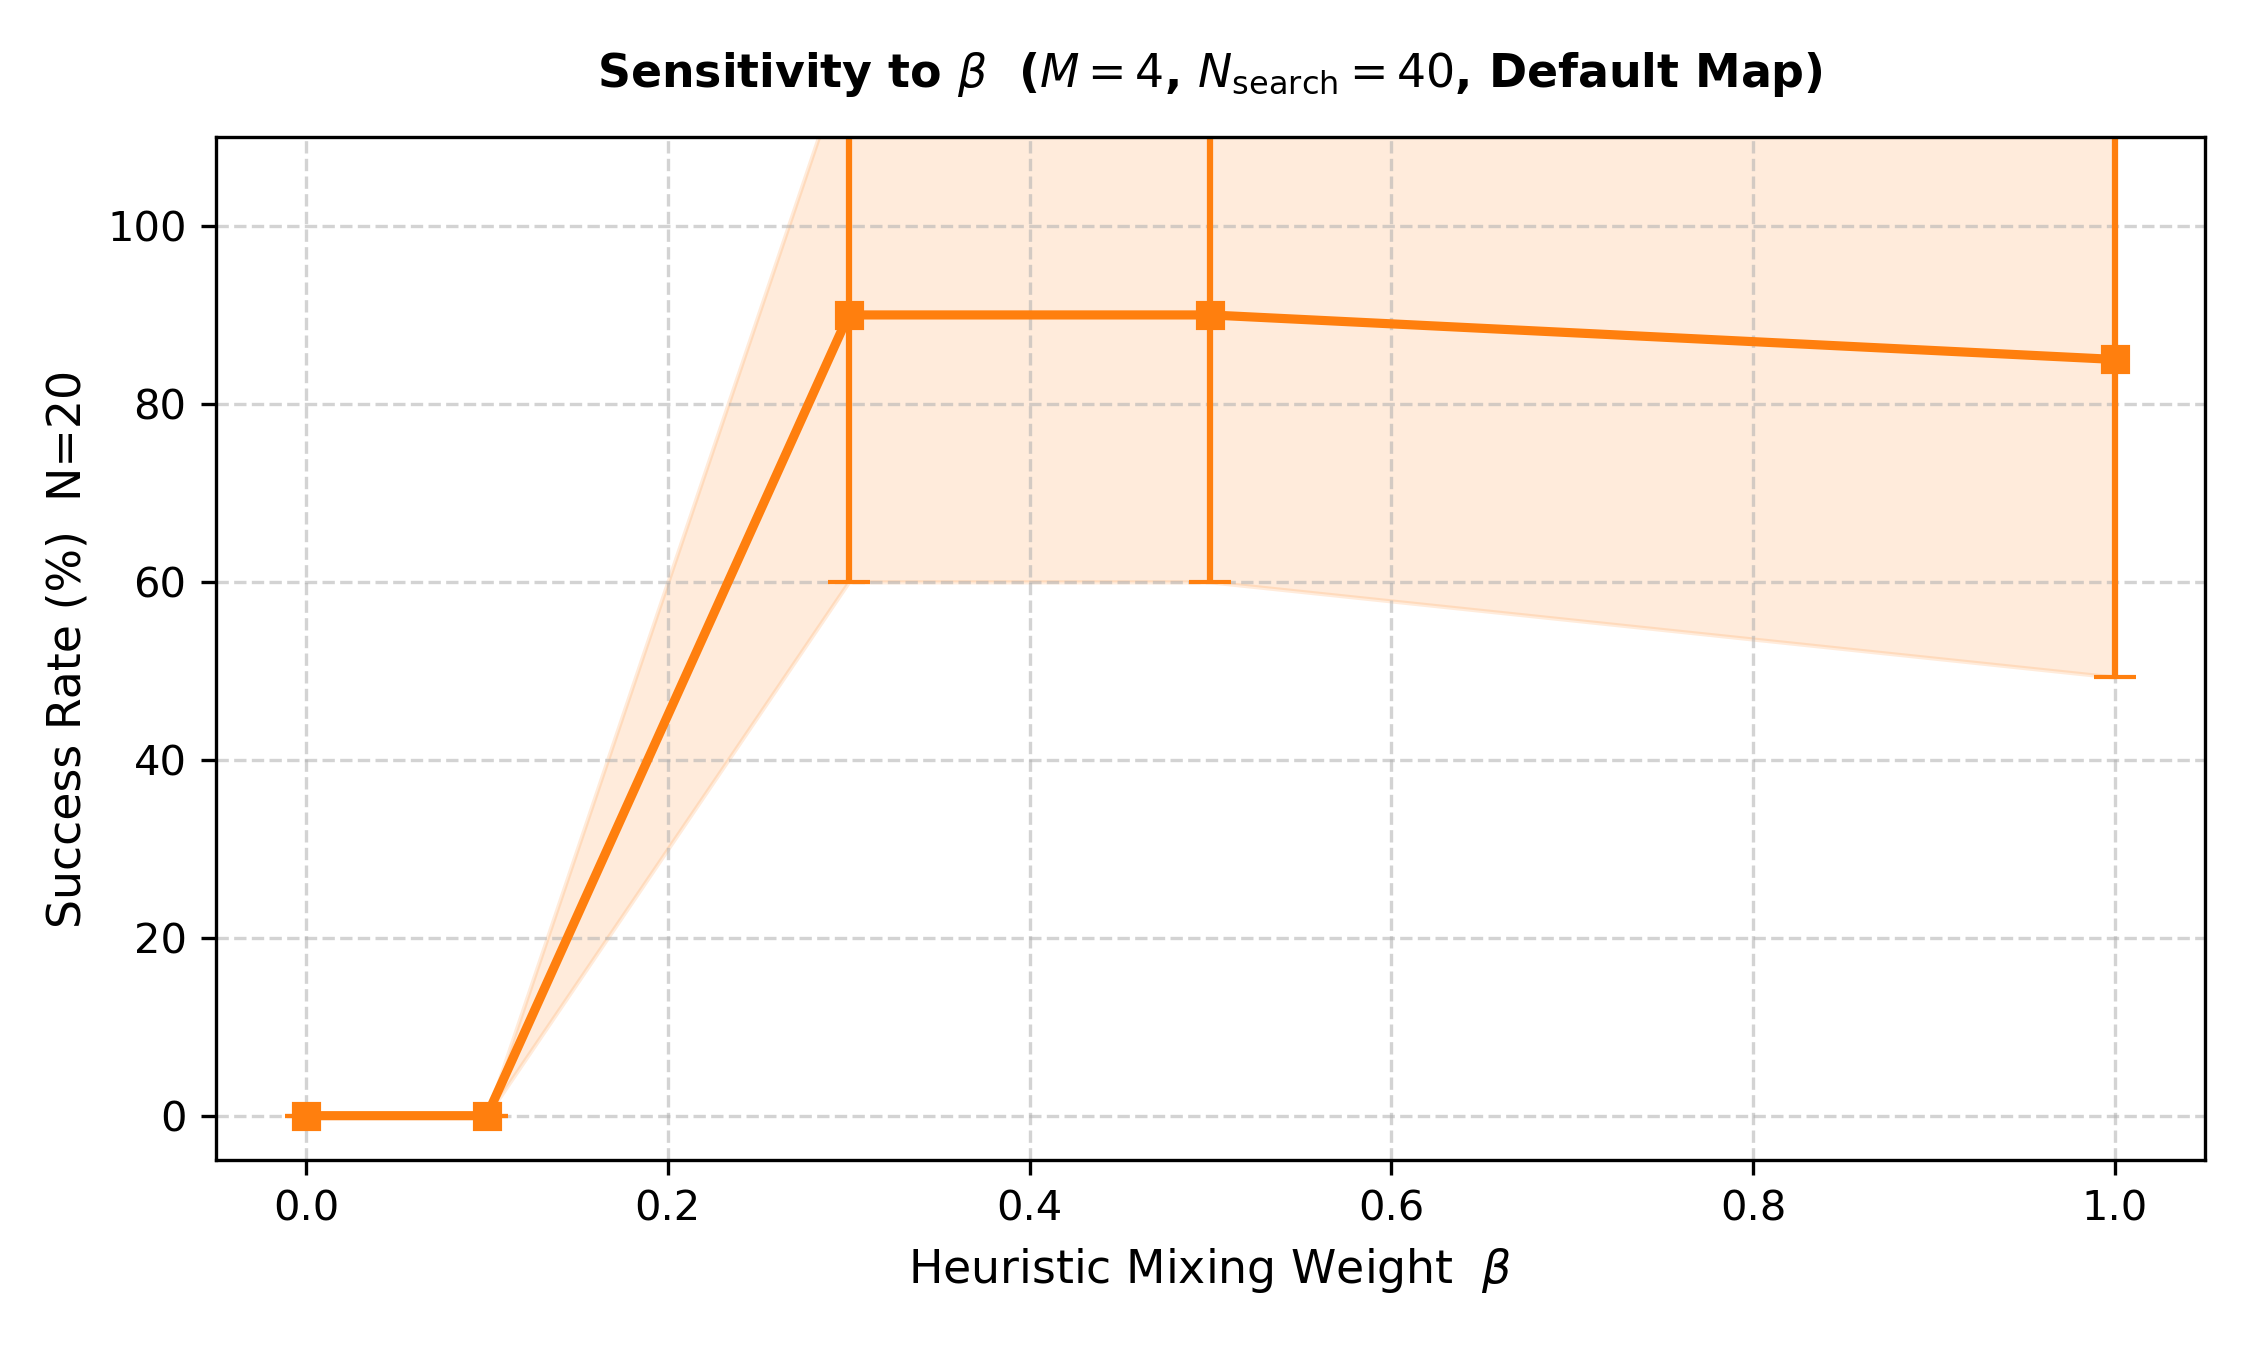
\includegraphics[width=0.48\textwidth]{results/beta_sensitivity.png}
\caption{Sensitivity to heuristic mixing weight $\beta$ ($M=4$, $N_{\rm search}=40$, $N=50$). Sharp threshold at $\beta=0.3$: below this the GNN prior fails to maintain goal-directedness and success collapses to $\le 2\%$.}
\label{fig:betasens}
\end{figure}

\subsection{Computational Complexity Analysis}
Running decentralized MCTS on independent agents reduces the computational scaling of joint action planning. Centralized joint-action planning scales exponentially at $O(|\mathcal{A}|^M) = O(8^M)$. In contrast, our decentralized planning framework scales linearly at $O(M \cdot N_{\mathrm{search}})$. Empirically, a single MCTS step with $N_{\mathrm{search}}=40$ takes $\approx 0.24$~s for $M=4$ agents on CPU, and $\approx 0.12$~s at $N_{\mathrm{search}}=20$. This linear scaling allows execution to remain feasible for larger agent counts, though at the expense of global coordination guarantees.

%===============================================================================
\section{Conclusion \& Future Work}
%===============================================================================
We presented a decentralized multi-agent coordination framework combining permutation-equivariant GNN architectures with Actor-Critic MCTS. Our experiments evaluate all configurations under a uniform sample size of $N=50$ randomised episodes per condition to ensure statistical uniformity, yielding four concrete empirical findings:
\begin{enumerate}
    \item \textbf{MCTS is non-negotiable}: GNN+1-step lookahead achieves exactly $0\%$ success across all agent counts, whereas PE-GNN+MCTS achieves $30$--$94\%$ on the Default Map, confirming that multi-step search is essential for resolving coordination bottlenecks.
    \item \textbf{Heuristic prior is necessary}: Below $\beta=0.3$ MCTS collapses to $\le 2\%$ success---the GNN prior alone cannot maintain goal-directedness within the search budget.
    \item \textbf{Theorem 4 is empirically validated}: $\hat{d}_{\min}$ decreases from $5.40$ (M=2) to $2.37$ (M=8) while the Theorem~4 bound grows from $0.686$ to $100.07$ and the failure rate ($1-$SR) increases monotonically from $6\%$ to $70\%$.
    \item \textbf{Zero-shot spatial generalisation}: A model trained on a $13{\times}13$ grid achieves a success rate of $94\%$ when transferred zero-shot to a $20{\times}20$ grid (an increase from $84\%$ on the trained grid layout), validating that spatial invariants scale effectively and that larger grids offer more room for conflict resolution.
\end{enumerate}
Key limitations and discussion:
\begin{itemize}
    \item \textbf{Communication range redundancy}: Our $R_c$ ablation on the $25{\times}25$ grid shows no degradation at $R_c = 3$ cells. This is because coordination events in this layout are inherently localized, meaning agents only need to communicate when in immediate proximity ($\le 3$ cells). Further studies are needed to evaluate performance in highly dense, bottlenecked corridors where long-range coordination might become active.
    \item \textbf{Static agent modelling in MCTS}: Treating other agents as static obstacles causes high-$M$ coordination failures. Extending to interactive or joint planning models would address this.
    \item \textbf{Sample size scaling}: While our uniform $N=50$ episodes provide statistically rigorous confidence intervals ($\pm 6.1\%$ width for $p=0.75$), future work should expand to $N \ge 100$ to further shrink error bounds.
\end{itemize}
Future work: (i) Rc-sparse attention via graph masking in the Transformer; (ii) interactive agent modelling in MCTS rollouts; (iii) continuous 3D robotic navigation benchmarks.

%===============================================================================
\begin{thebibliography}{99}

\bibitem{silver2017mastering}
D.~Silver et al., ``Mastering the game of Go without human knowledge,'' {\it Nature}, vol. 550, no. 7676, pp. 354--359, 2017.

\bibitem{kocsis2006bandit}
L.~Kocsis and C.~Szepesv{\'a}ri, ``Bandit based monte-carlo planning,'' in {\it ECML}, 2006, pp. 282--293.

\bibitem{bernstein2002complexity}
D.~S.~Bernstein, R.~Givan, N.~Immerman, and S.~Zilberstein, ``The complexity of decentralized control of Markov decision processes,'' {\it Mathematics of Operations Research}, vol. 27, no. 4, pp. 819--840, 2002.

\bibitem{sunehag2017value}
P.~Sunehag et al., ``Value-decomposition networks for cooperative multi-agent learning under shared sensory input,'' in {\it AAMAS}, 2018, pp. 2087--2089.

\bibitem{rashid2018qmix}
T.~Rashid et al., ``QMIX: Monotonic value factorization for deep multi-agent reinforcement learning,'' in {\it ICML}, 2018, pp. 4295--4304.

\bibitem{lowe2017multi}
R.~Lowe et al., ``Multi-agent actor-critic for mixed cooperative-competitive environments,'' in {\it NeurIPS}, 2017, pp. 6379--6390.

\bibitem{yu2021surprising}
C.~Yu et al., ``The surprising effectiveness of PPO in cooperative multi-agent games,'' {\it arXiv preprint arXiv:2103.01955}, 2021.

\bibitem{zaheer2017deep}
M.~Zaheer, S.~Kottur, B.~Ravanbakhsh, B.~Poczos, R.~R.~Salakhutdinov, and A.~J.~Smola, ``Deep sets,'' in {\it NeurIPS}, 2017, pp. 3391--3401.

\bibitem{lee2019set}
J.~Lee et al., ``Set Transformer: A framework for attention-based permutation-invariant neural networks,'' in {\it ICML}, 2019, pp. 3744--3753.

\bibitem{velickovic2018graph}
P.~Veli{\v{c}}kovi{\'{c}} et al., ``Graph Attention Networks,'' in {\it ICLR}, 2018.

\bibitem{sharon2015conflict}
G.~Sharon, R.~Stern, A.~Felner, and N.~R.~Sturtevant, ``Conflict-based search for optimal multi-agent pathfinding,'' {\it Artificial Intelligence}, vol. 219, pp. 40--66, 2015.

\bibitem{vandenberg2011reciprocal}
J.~van den Berg, S.~J.~Guy, M.~Lin, and D.~Manocha, ``Reciprocal $n$-body collision avoidance,'' in {\it Robotics Research}, Springer, 2011, pp. 3--19.

\bibitem{sartoretti2019primal}
G.~Sartoretti et al., ``PRIMAL: Pathfinding via reinforcement and imitation multi-agent learning,'' {\it IEEE Robotics and Automation Letters}, vol. 4, no. 3, pp. 2378--2385, 2019.

\bibitem{ma2021distributed}
Z.~Ma, Y.~Luo, and H.~Ma, ``Distributed heuristic multi-agent pathfinding with communication,'' in {\it ICRA}, 2021, pp. 1--7.

\bibitem{wang2023scrimp}
Y.~Wang et al., ``SCRIMP: Scalable communication for reinforcement- and imitation-learning-based multi-agent pathfinding,'' in {\it IROS}, 2023.

\end{thebibliography}

%===============================================================================
\appendix
\section{Detailed Mathematical Proofs}
%===============================================================================

\subsection{Proof of Theorem~\ref{thm:mcts_conv} (Decentralized MCTS Convergence)}\label{app:proof_mcts_conv}
We analyze convergence for a single agent $i$ planning at state $s$, under the assumption that other agents $j \neq i$ are modeled as static environmental obstacles within the search horizon. Under this assumption, the multi-agent Dec-POMDP transition dynamics $\mathcal{P}(s' \mid s, \mathbf{a})$ reduce to a stationary, single-agent Markov Decision Process (MDP) for agent $i$.
The selection rule of agent $i$ chooses action $a_t = \arg\max_{a} [Q^i(s, a) + U^i(s, a)]$ where $U^i(s, a) = c_{\mathrm{puct}} P^i(s, a) \frac{\sqrt{N(s)}}{1 + N(s, a)}$ and $N(s) = \sum_{a'} N(s, a')$.
First, we show that all valid actions are selected infinitely often as $N(s) \to \infty$. Suppose there exists a suboptimal action $a$ selected only a finite number of times, so that $\dots, \lim_{t\to\infty} N_t(s, a) = C_a < \infty$. The exploration term for action $a$ grows as $U_t(s, a) = O(\sqrt{t}) \to \infty$ as $t \to \infty$, while the exploration term for the infinitely selected optimal action $a^*$ decays as $U_t(s, a^*) \to 0$. Since the estimated value $Q(s, a)$ is bounded in $[-1, 1]$, the selection index of action $a$ will eventually exceed that of $a^*$, leading to a contradiction.
By the Strong Law of Large Numbers, since all actions are visited infinitely often, the running action-value estimates $Q^i(s, a)$ converge almost surely to the true action values $Q^*(s, a)$. The visit counts of suboptimal actions grow sublinearly at $O(\sqrt{t})$ because the selection index condition requires $U_t(s, a) \geq \frac{1}{2} \Delta_a$, which bounds $1 + N_t(s, a) \leq 2 c_{\mathrm{puct}} P(s, a) \sqrt{t} / \Delta_a$. Thus, as temperature $\tau \to 0$, the visit frequency converges to a point mass on the optimal local best response.

\subsection{Proof of Theorem~\ref{thm:safety_guar} (Local Safety Guarantee)}\label{app:proof_safety_guar}
Assume that the KL divergence between the coordinated potential field heuristic $P_H^i$ and the policy $\pi_\theta^i$ is bounded:
\begin{equation}
    D_{KL}(P_H^i \parallel \pi_\theta^i) \leq \epsilon
\end{equation}
By expanding the definition of Kullback-Leibler divergence, we write:
\begin{equation}
    \sum_{a \in \mathcal{A}} P_H^i(a \mid s) \log\left(\frac{P_H^i(a \mid s)}{\pi_\theta^i(a \mid s)}\right) \leq \epsilon
\end{equation}
Since all terms in the summation are non-negative, any single action $a$ must satisfy:
\begin{equation}
    P_H^i(a \mid s) \log\left(\frac{P_H^i(a \mid s)}{\pi_\theta^i(a \mid s)}\right) \leq \epsilon
\end{equation}
For any safe action $a$ satisfying the heuristic threshold $P_H^i(a \mid s) \geq p_{\min} > 0$:
\begin{equation}
    p_{\min} \log\left(\frac{p_{\min}}{\pi_\theta^i(a \mid s)}\right) \leq \epsilon
\end{equation}
Rearranging the terms:
\begin{equation}
    \log\left(\frac{p_{\min}}{\pi_\theta^i(a \mid s)}\right) \leq \frac{\epsilon}{p_{\min}} \implies \frac{\pi_\theta^i(a \mid s)}{p_{\min}} \geq \exp\left(-\frac{\epsilon}{p_{\min}}\right)
\end{equation}
Multiplying by $p_{\min}$ yields the probability lower bound:
\begin{equation}
    \pi_\theta^i(a \mid s) \geq p_{\min} \cdot \exp\left(-\frac{\epsilon}{p_{\min}}\right) > 0
\end{equation}
This guarantees that safe actions, as defined by the potential field heuristic, retain a strictly positive selection probability, ensuring safety during exploration.

\subsection{Proof of Theorem~\ref{thm:value_decomp} (Equivariant Additive Value Decomposition)}\label{app:proof_value_decomp}

\paragraph{Part 1: Equivariance.}
The value head is a linear map $W_V: \mathbb{R}^d \to \mathbb{R}$ applied row-wise to the GNN output $f_\theta(Z) \in \mathbb{R}^{M \times d}$, giving $V_i(s) = W_V^\top [f_\theta(Z)]_i$. By Theorem~\ref{thm:perm_equiv}, $f_\theta(P_\sigma Z) = P_\sigma f_\theta(Z)$ for any $\sigma \in S_M$. Since $P_\sigma$ merely reorders the rows:
\begin{equation}
    V_{\sigma(i)}(P_\sigma s) = W_V^\top [P_\sigma f_\theta(Z)]_{\sigma(i)} = W_V^\top [f_\theta(Z)]_i = V_i(s)
\end{equation}
which establishes the equivariance property. \hfill $\square$

\paragraph{Part 2: Decomposition Error Bound.}
Write the joint value as a sum of individual and interaction terms:
\begin{equation}
    V_{\mathrm{joint}}(s) = \mathbb{E}_\pi\left[\sum_{t=0}^{\infty} \gamma^t \left(\sum_{i} r_i(s_t, a_{t,i}) + \sum_{i<j} r_{ij}(s_{t,i}, s_{t,j}, a_{t,i}, a_{t,j})\right) \Bigg| s_0 = s\right]
\end{equation}
Under decentralized execution, each agent optimizes $V_i(s) = \mathbb{E}_{\pi_i}\left[\sum_{t=0}^{\infty} \gamma^t r_i(s_t, a_{t,i}) \mid s_{t,i} = s_i\right]$, capturing only individual rewards. The decomposition error is therefore:
\begin{align}
    \left| V_{\mathrm{joint}}(s) - \sum_{i=1}^M V_i(s) \right| &= \left| \mathbb{E}_\pi\left[\sum_{t=0}^{\infty} \gamma^t \sum_{i<j} r_{ij}(s_{t,i}, s_{t,j}, a_{t,i}, a_{t,j}) \right] \right| \\
    &\leq \sum_{t=0}^{\infty} \gamma^t \sum_{i<j} \mathbb{E}\left[|r_{ij}(s_{t,i}, s_{t,j}, a_{t,i}, a_{t,j})|\right]
\end{align}
Applying the pairwise interaction decay assumption $|r_{ij}| \leq C / (d(s_i, s_j))^\alpha$ and the fact that spatial distances are lower bounded by $d_{\min}(s)$ in state $s$:
\begin{equation}
    \leq \sum_{t=0}^{\infty} \gamma^t \cdot \binom{M}{2} \cdot \frac{C}{(d_{\min}(s))^\alpha} = \frac{C \binom{M}{2}}{(1-\gamma)(d_{\min}(s))^\alpha}
\end{equation}
where we used $\sum_{t=0}^{\infty} \gamma^t = 1/(1-\gamma)$. This completes the proof. \hfill $\square$

\begin{remark}[Tightness of the Bound]
The bound is tight up to constants in the limit $d_{\min}(s) \to 0$ (crowded states), where pairwise interactions dominate and value decomposition breaks down. Conversely, as $d_{\min}(s) \to \infty$ (well-separated agents), the bound approaches zero and the decentralized estimates sum exactly to the joint value. The $\binom{M}{2}$ factor confirms the quadratic growth of coordination complexity with agent count, consistent with the empirical scalability cliff in Section~\ref{sec:experiments}.
\end{remark}

\subsection{Numerical Verification of Permutation Equivariance}\label{app:numerical_equiv}
To confirm Theorem~\ref{thm:perm_equiv} holds in practice, we numerically evaluated the maximum absolute difference between $f_\theta(P_\sigma Z)$ and $P_\sigma f_\theta(Z)$ over 50 random permutations $\sigma \in S_4$ applied to random input matrices $Z \in \mathbb{R}^{4 \times 128}$. The results are summarized in Table~\ref{tab:equiv_check}.

\begin{table}[H]
\centering
\small
\begin{tabular}{|l|c|}
\hline
\textbf{Metric} & \textbf{Value} \\
\hline
Max absolute difference $\|f_\theta(P_\sigma Z) - P_\sigma f_\theta(Z)\|_\infty$ & $7.15 \times 10^{-7}$ \\
Mean absolute difference & $4.20 \times 10^{-7}$ \\
\hline
\end{tabular}
\caption{Numerical Equivariance Verification ($M=4$, 50 random permutations)}
\label{tab:equiv_check}
\end{table}
Differences on the order of $10^{-7}$ are attributable solely to IEEE 754 floating-point rounding and confirm that the implementation satisfies equivariance to machine precision.

\end{document}
